%!TeX program = lualatex

\documentclass[oneside]{academica}
\input{preamble}

\overtitle{notes for}
\title{Network Security}
\author{Filippo Merlo}
\date{2023-2024}

\begin{document}

\frontmatter

\maketitle

\tableofcontents

\mainmatter

\chapter{Introduction}

Cybersecurity can be split into:
\begin{itemize}
  \item \textbf{information security}: security of the data
  \item \textbf{network security}: protection of services and means of data sharing, also from a performance/availability point of view
\end{itemize}

\section{Security Objectives}

The main security objectives are:

\begin{itemize}
  \item \textbf{Confidentiality}, which is the combination of

  \begin{minipage}{0.63\textwidth}
        \begin{itemize}
          \item \textbf{data confidentiality}: assures that private/confident information are not made available.
          \item \textbf{privacy}: assures that individuals control which information about them is collected, where is stored and who can read it.
        \end{itemize}
  \end{minipage}
  \hfill
  \begin{minipage}{0.33\textwidth}
    \centering
    \vspace{-10pt}
    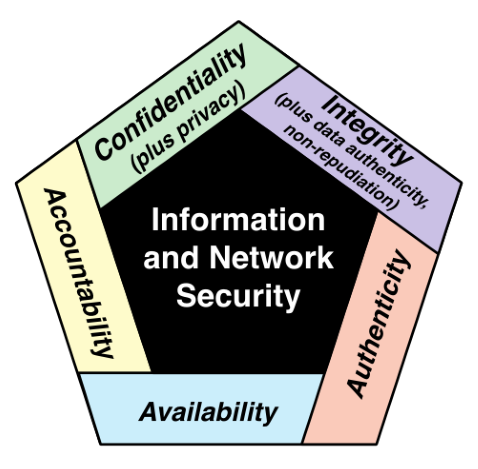
\includegraphics[width=0.8\linewidth]{figures/ciaaa}
  \end{minipage}

  \item \textbf{Integrity}, none can change the data and this is assured with:
    \begin{itemize}
      \item \textbf{data integrity}: data and programs are changed only via authorized access. It encompasses data authenticity and non-repudation.
      \item \textbf{system integrity}: assures that a system performs its intended function without any possible manipulation, \textit{e.g.} trying to manipulate data.
    \end{itemize}
  \item \textbf{Authenticity}: being able to be verified and trusted \textit{e.g.} validity of a transmission.
  \item \textbf{Availability}
  \item \textbf{Accountability}: being able to trace the author of an action. This security objective provides also:
    \begin{itemize}
      \item non-repudiation
      \item intrusion detection and prevention
      \item deterrence
      \item fault isolation
    \end{itemize}
    Systems must keep records of any specified activity, to know who have done what and when, thus, after an attack, being able also to find how someone did something malicious, although not always possible, in order to implement a patch.
\end{itemize}

\section{Security Challenges}

There are a lot of security challenges, and one of the most important is \textbf{implementation}, because is not easy to implement exactly what a system should do without telling him what he can't do and we can't implement a system using negations (\textit{e.g.} you cannot do that if this or that, $\ldots$) because we can't cover all possible cases.
Imagine this like a non-deterministic Turing Machine where we have a lot of NO cases and only few, if any, YES cases.
This translates in a huge work trying to implement all possible negation cases.

Other security challenges are:
\begin{itemize}
  \item constant monitoring cost
  \item security is seen as an impediment for efficiency and user-friendliness
  \item often seen as ``not needed'' until something goes wrong
\end{itemize}

Because security isn't simple but heavy, there are risk management procedures in order to deal with security while maintaining certain performance standards, lowering the risk as much as possible without hurting too much other area (performance, ecc).
Security costs but accidents cost more, and even only one bad event can be so critical that will cost the shut down of a service or a facility.

\section{Security Architecture}

\begin{itemize}
  \item Security \textbf{attack}
  \item Security \textbf{mechanism}: process to detect, prevent or recover an attack.
  \item Security \textbf{service}: service that enhances security of data processing and information transfer. It counters security attacks by merging different security mechanisms.
\end{itemize}

\subsection{Security Attacks}
Security attacks can be:
\begin{itemize}
  \item \textbf{Passive}: these don't affect the system resources, because its scope is to gain information. Are impossible to detect because the system behaves normally. An example is traffic analysis.
  \item \textbf{Active}: these alter some data or affect system's functioning. Almost impossible to prevent, in fact the goal is to detect an attack and be able to delay/isolate it as much as possible, while trying to patch it. Some examples are:
    \begin{itemize}
      \item \textit{Masquerade}: one entity pretends to be a different entity.
      \item \textit{Replay}: retransmission of data, usually follows a passive attack.
      \item \textit{Data Modification}: alteration, reordering or delay of some data.
      \item \textit{DoS\footnote{Denial of Service}}: prevents/inhibits the normal state of a system.
    \end{itemize}
\end{itemize}

\subsection{Security Mechanisms}

\begin{itemize}
  \item \textbf{Cryptographic algorithms}:
    \begin{itemize}
      \item \textit{reversible}: encryption/decryption with a key
      \item \textit{irreversible}: algorithm that only encrypts because it cannot be reverted/decrypted, like HASH functions, pretty useful for digital signature and authentication
    \end{itemize}
  \item \textbf{Data integrity}
  \item \textbf{Digital signature}: used to check integrity by appending some data to a message or by transforming the data (HASH).
  \item \textbf{Authentication exchange}: ensure the identity of an entity by means of information exchange.
  \item \textbf{Traffic padding}: insertion of bits between data streams in order to generate noise to protect against traffic analysis. An attacker should not be able to distinguish noise from real data.
  \item \textbf{Routing control}: allows routing changes to avoid certain routes for security reasons, \textit{i.e.} use only certain pre-selected routes, \textit{e.g.} Samsung avoids routes through Apple's routers.
  \item \textbf{Notarization}: use of a trusted third party to assure certain properties of a data exchange.
  \item \textbf{Access control}: enforces access rights to resources, \textit{e.g.} think about file modes (chmod).
\end{itemize}

\subsection{Security Services}

\subsubsection{Authentication}

Is concerned with assuring that a communication is authentic covering
\begin{itemize}
  \item message: assures that a message really comes from where it claims to be from
  \item interaction: assures that the two entities are authentic and that the connection is not interfered
\end{itemize}
We have two specific authentication services:
\begin{itemize}
  \item \textbf{Peer entity authentication}: provides for the corroboration of the identity of a peer entity in an association. Two entities are considered peers if they implement the same protocol in different systems.
  \item \textbf{Data origin authentication}: provides only for the corroboration of the source of a data unit.
\end{itemize}

\subsubsection{Access Control}

Provides the ability to limit and control the access to host systems and applications by first identifying the entity of who is trying to gain access.

\subsubsection{Data Confidentiality}

Consists in the protection of transmitted data from passive attacks (\textit{e.g.} XML encryption) and prevents the unauthenticated analysis of traffic flow (metadata protection \textit{e.g.} emails' header)

\subsubsection{Data integrity}

\begin{itemize}
  \item \textbf{Connection-oriented integrity service}: deals with \textbf{stream} of messages and it assures that the whole stream is received as sent with no modification whatsoever (\textit{e.g.} duplication, insertion, modification, reordering, or replay).
  \item \textbf{Connectionless integrity service}: deals with \textbf{individual} messages, protecting them against data modification.
\end{itemize}

\subsubsection{Non-Repudation}

Prevents either sender or receiver from denying a transmitted message.
Both parties can prove that the message has been sent and received.
In this case the attacker is one of the two parties and he's aiming at altering metadata, to falsify a certain communication.
Non-repudation encloses also authentication for obvious reasons.
However, the main difference between non-repudation and authentication is that the latter is done between the two parties, while in non-repudation the authentication part is necessary to prove a communication to a third party, \textit{e.g.} Bob can show everyone that Alice has sent him a message at a specific time.

\subsubsection{Availability}

Ensures a systems' availability by protecting against DoS attacks or high-traffic time slots, implementing a proper management of the systems' resources (\textit{e.g.} load balancer).
For high-traffic time slots imagine the load over Netflix servers on a Saturday evening.

\subsection{Cryptographic Algorithms}

Cryptographic algorithms can be split among:
\begin{itemize}
  \vspace{-5pt}
  \item \textbf{Keyless}: these are deterministic functions that have certain properties useful for cryptography, \textit{e.g.} hash functions, like MD5 and SHA, and PRNG\footnote{Pseudo Random Number Generator}.
    Hash functions turn a variable amount of text into a small, fixed-length value called \textbf{digest}.
    However, not all hash functions are cryptographically secure, because they need the following additional properties:
    \vspace{-5pt}
    \begin{enumerate}
      \item given $h \in 2^*$, find $x \in 2^*$ s.t. $H(x) = h$
      \item given $x \in 2^*$, find $y \neq x$ s.t. $H(y) = H(x)$
      \item find $x, y$ s.t. $H(x) = H(y)$
    \end{enumerate}
  \vspace{-5pt}
  \item \textbf{Single key}: are called \textbf{symmetric} algorithms, because the same key is used both for encryption and decryption and can be further split into
    \vspace{-5pt}
    \begin{itemize}
      \item \textit{block} ciphers: chunks of bits
      \item \textit{stream} ciphers: sequence of bits
    \end{itemize}
    Another single key algorithm is \textbf{MAC}\footnote{Message Authentication Code} and is the composition of a hash function plus a key.
    When is sent a message is also sent its digest (output of the MAC).
    In this way, if we have the key, we can verify the integrity of the message, by applying the MAC algorithm with the key over the message and check if our MAC output is equal to the digest received.
  \item \textbf{Double key}: are called \textbf{asymmetric} algorithms, because the mechanism of encryption and decryption is different: different operations and different key.
    These algorithms are useful for different applications:
    \begin{itemize}
      \item \textit{Digital signature}: a digital signature is a value computed with a cryptographic algorithm and associated with a data object in such a way that any recipient of the data can use the signature to verify the data’s origin and integrity.
        This implements non-repudation, which implies authentication.
      \item \textit{Key exchange}: the process of securely distributing a symmetric key to two or more parties.
      \item \textit{User authentication}: the process of authenticating that a user attempting to access an application or service is genuine and, similarly, that the application or service is genuine.
        This is different from digital signature because is relative to a \textit{temporary} session.
    \end{itemize}
\end{itemize}

\section{Security Design Principles}

\begin{itemize}
  \item \textbf{Economy of mechanism}: the design of security measures for both software and hardware should be as simple (and small) as possible, because in complex implementations there are more opportunities for an adversary to discover weaknesses to exploit.
  \item \textbf{Fail-safe defaults}: access should be implemented based on \textbf{permission} rather than exclusion, thus the default situation is a lack of access and then for each entity are added above certain permissions for certain conditions, \textit{i.e.} everything that is not specifically allowed is denied.
  \item \textbf{Complete mediation}: every access must be checked against the access control mechanism, and the access decision should not be cached, but instead should be evaluated for each access.
    However, this is resource intensive, thus are used other approaches.
  \item \textbf{Open design}: the design of a security mechanism should be open rather than secret, even cryptographic algorithms.
  \item \textbf{Separation of privilege}: is a good practice to use multiple privilege attributes to achieve access to a restricted resource, instead of using a single special attribute for that special access, \textit{i.e.} small different checks are better than a single big/strong check.
  \item \textbf{Least privilege}: every process and every user of the system should operate using the least amount of privileges necessary to perform the task.
    This principle usually implements \textbf{role-access} control, where each role have its own permissions.
  \item \textbf{Least common mechanism}: the design should minimize the functions shared by different users, providing mutual security, \textit{i.e.} from outside users cannot access resources which aren't theirs.
    This differs from isolation because isolation acts over the separation of component of a system.
  \item \textbf{Psychological acceptability}: implies that the security mechanisms should not interfere unduly with the work of users and not being intrusive or burdensome, \textit{i.e.} user-friendly with the least obstruction/friction possible.
  \item \textbf{Isolation}: different layers of isolation to prevent disclosure or tampering.
  \item \textbf{Encapsulation}: is a specific form of isolation where procedures and data objects are encapsulated under a domain of the system that owns them. In this way, data are only accessible using the procedures of the protected subsystem, and those may be called only at designated domain entry points.
  \item \textbf{Modularity}: consists in the development of security functions as separate, protected modules from the actual components, \textit{e.g.} authentication implemented as a component and the application implemented as a different component.
    This design allows also an easier process for fixing problems when they arise, because we can work directly on the component that is affected by the problem.
  \item \textbf{Layering}: refers to the use of multiple, overlapping protection mechanisms, thus in case of failure of a certain mechanism, the whole system isn't vulnerable because to be vulnerable it means that all mechanisms together has been disrupted.
    An example is two-factor authentication, which is a 2-layered mechanism.
  \item \textbf{Least astonishment}: means that a program should act as the user may expect, so always respond in a way that is least likely to astonish/surprise the user. Vice versa the user should have the correct overview of what is the security level, so it should not be surprised when asked about something.
\end{itemize}

\section{Attack Surfaces}

\textbf{Attack surface} consists of the reachable and exploitable vulnerabilities in a system, \textit{e.g.} open ports or the services under a firewall, and its main categories are:
\begin{itemize}
  \item \textbf{Network attack} surface: vulnerabilities over wide-area network, or the Internet.
  \item \textbf{Software attack} surface: vulnerabilities in applications, where particularly important cases are web servers and browsers.
  \item \textbf{Human attack} surface: personnel is also a vulnerability because can be physically attacked or can be influenced through social engineering.
\end{itemize}

An \textbf{attack surface analysis} is a useful technique for assessing the scale and severity of threats to a system.
After an analysis, designers should find ways/fixes to reduce the surface attack, starting from the major threats on important data.

\newpage

\begin{figure}[h]
  \begin{center}
    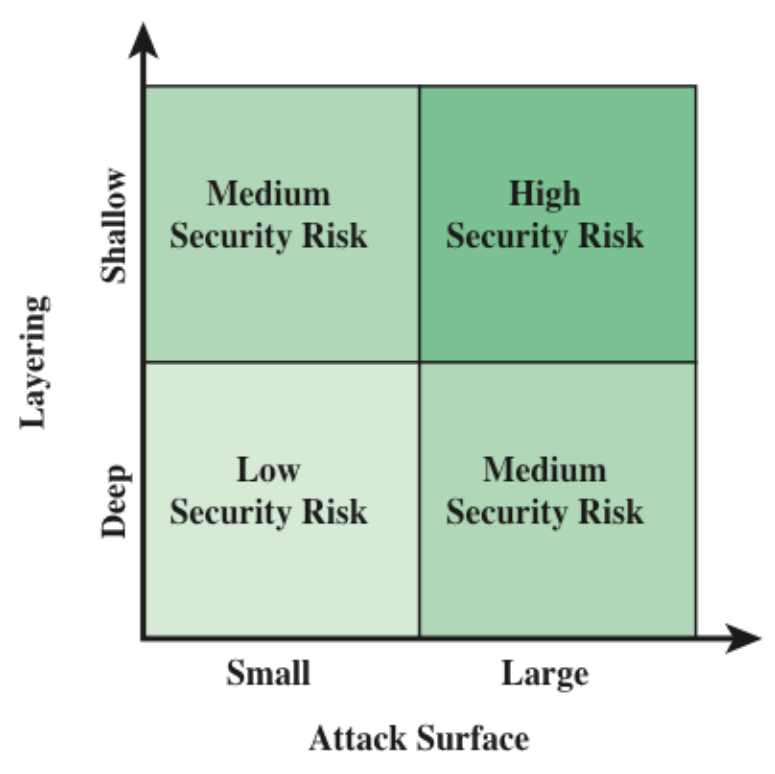
\includegraphics[width=0.35\linewidth]{figures/attack_surface}
  \end{center}
\end{figure}

An \textbf{attack tree} is a branching, hierarchical data structure that represents a set of potential techniques for exploiting security vulnerabilities.
The \textbf{security incident} that we want to avoid is the root of the tree.
Each leaf of the tree represents a possible way to start an attack that can lead to the incident.
The motivation behind attack trees is to effectively exploit the information available on \textbf{attack patterns}.

For each node can be associated different labels, for example
\begin{itemize}
  \item ``chances level'' that the attack can be performed
  \item cost of such an attack
  \item special equipment/situation requirements to be able to perform the attack
\end{itemize}
and all the labels help us to highlight certain paths among all possible.

The attack tree is really useful to have an overview of the possible threats paths and so it guides us in the design of systems and applications, helping in making the right choice (and strength) of countermeasures.

\section{Network Security}

\subsection{Security Model}

The \textbf{Dolev-Yao model} (figure~\ref{fig:dolev_yao_model}) defines network security, and shows us there are four basic tasks in designing a particular security service:
\begin{enumerate}
  \item Designing an \textit{algorithm} for the security related transformations
  \item Generate the \textit{secret information} that the algorithm need
  \item \textit{Distribution} of the secret information
  \item Specify a \textit{protocol} that sender and receiver can use to combine the algorithm with the secret information and so being able to achieve a particular security service.
\end{enumerate}

\begin{figure}[h]
  \begin{center}
    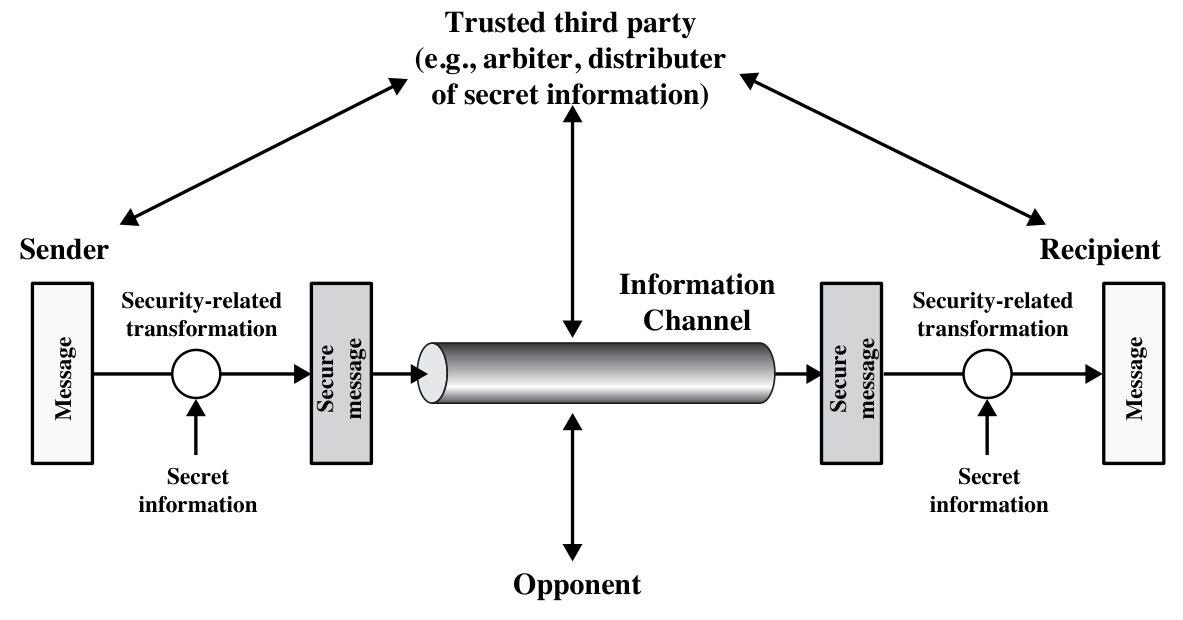
\includegraphics[width=0.7\linewidth]{figures/dolev_yao_model}
  \end{center}
  \caption{Dolev-Yao model}\label{fig:dolev_yao_model}
\end{figure}

\subsection{Communication Security}

Communication security deals with the protection of communications through the network, including measures to protect against both passive and active attacks.
It is primarily implemented using network protocols, which defines the structure of the individual data units and the control commands that manage the data transfer.

\subsubsection{Encryption}

To protect communications, following the Dolev-Yao model, we need to apply encryption to each layer of the TCP/IP stack.
Communication encryption happens in two ways:
\begin{itemize}
  \item \textbf{link encryption}: encryption occurs independently on every connection link, all over the multiple links in the network.
  \item \textbf{end-to-end encryption}: it occurs between original source and final destination, thus both devices at each end must share a key. Not the whole frame is encrypted, because the header must remain in clear, otherwise routers doesn't know where to send it.
\end{itemize}

The encryption on each layer is different, in fact:
\begin{itemize}
  \item \textit{layer 1} (physical): physical protection of the cable, making it inaccessible from outside.
    However, physical protection is not always possible, for example the electromagnetic waves of a wireless connection, and when possible is expensive to implement.
  \item \textit{layer 2} (datalink): aim to protect the frame data and is implemented in network cards (protocols like WEP or WPA). The frame header is obviously left in clear. Data are still vulnerable in network bridges (routers).
  \item \textit{layer 3} (network/IP): is implemented in the kernel and leaves unencrypted only the IP. A protocol that does this is IPsec, which integrates IP with authentication and confidentiality. In this layer are also implemented VPNs.
  \item \textit{layer 4} (transport/TCP/UDP): encryption is implemented through libraries or system's API. The main protocol of this layer is TLS/SSL.
  \item \textit{layer 5} (application): are end-to-end encrypted services, because encryption is implemented directly in applications, thus each one has their own security protocol, \textit{e.g.} SSH, PGP, PEC, OAuth2, $\ldots$
\end{itemize}

\subsubsection{Standards}

The NIST\footnote{National Institute of Standards and Technology} is a U.S. federal agency that deals with standards, while ISO\footnote{Internet Society} does the same but is a worldwide organization.

\subsection{Device Security}

Network security protects also network devices, such as routers and switches, and end systems connected to the network, like clients or servers.
There are 3 possible security device's types:
\begin{enumerate}
  \item \textbf{Firewall}: a hardware and/or software capability that limits access between a network and device attached to the network, in accordance with a specific \textit{security policy}. Acts like a \textbf{filter} that permits or denies data traffic.
  \item \textbf{Intrusion detection}: hardware or software that monitor the network/communications to provide real-time warning of unauthorized access to system resources.
  \item \textbf{Intrusion prevention}: hardware or software designed to
    \begin{itemize}
      \item detect intrusive activity
      \item attempt to stop the activity
    \end{itemize}
\end{enumerate}

\chapter{Message Authentication}

The requirements for message authentication are to be secure against:
\begin{itemize}
  \item \textbf{masquerading}, \textit{i.e.} insertion of messages into a network from a fraudulent source
  \item content/sequence/timing \textbf{modification}
  \item source/destination \textbf{repudiation}
\end{itemize}

\section{Functions}

Message authentication functions implements authentication in two ways:
\begin{itemize}
  \item \textbf{low-level}: there must exist a function that \textit{produces} an authenticator and a function that \textit{verifies} it.
  \item \textbf{high-level}: uses lower-level functions as primitives in an authentication protocol.
\end{itemize}
Some example of functions are hash functions, cryptographic functions (also used for message encryption) or MAC\footnote{Message Authentication Code}.
The difference between Hash and MAC is only that the latter uses a secret key.

\subsection{Hash Functions}

Usually the message to send, before being encrypted, is concatenated with a \textbf{control code}, generated for example using CRC or checksum, that is used by the receiver to detect transmission errors, \textit{i.e.} if the CRC of the received message content and the received CRC doesn't match it means that the message is compromised (transmission error or manipulation attempt).

Another possible use case is that we calculate the control code of the message, then we encrypt only the message content and finally we concatenate them.
In this way we cut out the additional cost of encryption of the control code, while maintaining the security of the control code.

\begin{note}
  If the control code is calculated after message encryption and concatenated, it becomes useless because if an attacker can just create a new message, encrypt it and then it can calculate the control code.
  The receiver would not know that the message has been completely substituted, because this approach is vulnerable against MITM.
\end{note}

\subsection{Cryptographic Functions}

Cryptographic functions can be used for implementing:
\begin{itemize}
  \item \textit{symmetric} encryption $\rightarrow$ confidentiality and authentication
  \item \textit{asymmetric public-key} encryption $\rightarrow$ confidentiality
  \item \textit{asymmetric private-key} encryption $\rightarrow$ authentication and signature
\end{itemize}
As we can see, to achieve the same security of symmetric encryption, we have to combine, in order, asymmetric private and public encryption, and this implies that using the second approach is more resource expensive, without even taking into account that asymmetric encryption is by several orders slower than symmetric one.

\subsection{MAC}

The message to send is concatenated with a MAC code, which is encrypted with its own key.
Depending on the situation we can have 3 cases:
\begin{enumerate}
  \item plain message concatenated with MAC
  \item previously encrypted message concatenated with MAC
  \item plain message concatenated with MAC, then overall message is encrypted
\end{enumerate}
In each case the MAC is always been encrypted before with its own key.
\\\\
Some variant of MAC are:
\begin{itemize}
  \begin{minipage}{0.52\textwidth}
    \item \textbf{HMAC}: the motivation behind is that hash functions are faster than symmetric encryption.
      The strength of HMAC is strictly dependent on the strength of the underlying hash function (we can reduce hash to HMAC ?).
    \item \textbf{CBC-MAC\footnotemark{}}: uses some cryptographic function to encrypt in chaining mode all the data, until the end.
      The last block obtained is the authentication tag $t$.
      Used for example in IPsec and TLS.
      CBC-MAC is secure until we use fixed-length messages, while using \textbf{variable-length} ones becomes unsecure.
      In fact, an attacker who knows the correct authentication tag pairs for two messages $(m,t)$ and $(m^\prime,t^\prime)$ can generate a new message $m^{\prime\prime}$ s.t. it has the same CBC-MAC $t^\prime$ of $m^\prime$, \textit{i.e.} is able to create a new valid pair $(m^{\prime\prime}, t^\prime)$.
  \end{minipage}
  \hfill
  \begin{minipage}{0.34\textwidth}
      \centering
      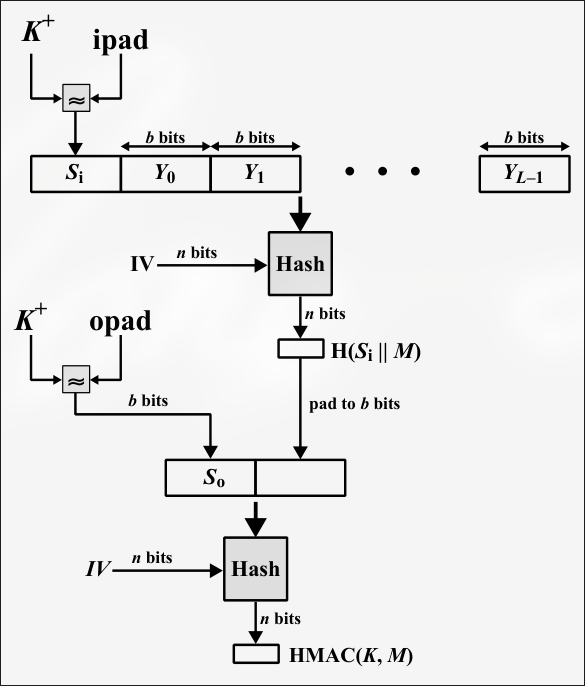
\includegraphics[width=\linewidth]{figures/hmac}
      \captionof*{figure}{HMAC structure}
  \end{minipage}
  \footnotetext{Cipher Block Chaining MAC}
    That's because, by forging a message $m^{\prime\prime}$ with the following structure
    \begin{equation*}
      m^{\prime\prime} = m \Vert \left( m_1^\prime \oplus t \right) \Vert m_2^\prime \Vert \ldots \Vert m_i^\prime
    \end{equation*}
    by computing the CBC-MAC for it, the tag $t$ gets cancelled out and thus also $m$.
  \item \textbf{CMAC\footnotemark}: tries to fix CBC-MAC chaining vulnerability (as just shown with a length attack).
    It works like CBC-MAC, but at the end of the encryption, CMAC XORs the final block with a secret value, called \textbf{tweak}, which is derived from the key.
    This ensures that the final block is treated differently from the other blocks, so that an attacker can no more exploit this vulnerability as an oracle for building new messages.
\end{itemize}
\footnotetext{Cipher-based MAC}

\section{AE - Authenticated Encryption}

Is a term used to describe encryption systems that simultaneously protect confidentiality and authenticity of communications, through one of the following approaches:
\begin{itemize}
  \item hashing followed by encryption
  \item authentication followed by encryption (MtE)
  \item encryption followed by authentication (EtM)
  \item independently encrypt and authenticate (E\&M)
\end{itemize}
None of the following approaches is completely secure, because each one has its own flaws.

\subsection{MtE - MAC then Encrypt}

\begin{minipage}{0.58\textwidth}
  A MAC is produced based on the plaintext, then the plaintext and MAC are together encrypted to produce a ciphertext based on both.
  Is sent the encrypted message that contains both the data and the MAC.
  Has been used in SSL/TLS until version 1.2, where, even though MtE is not strongly unforgeable in itself, through TLS implementation it were strongly unforgeable (as it been proved by Krawczyk).
  This approach however is also vulnerable against padding oracle attacks.
\end{minipage}
\hfill
\begin{minipage}{0.38\textwidth}
  \begin{center}
    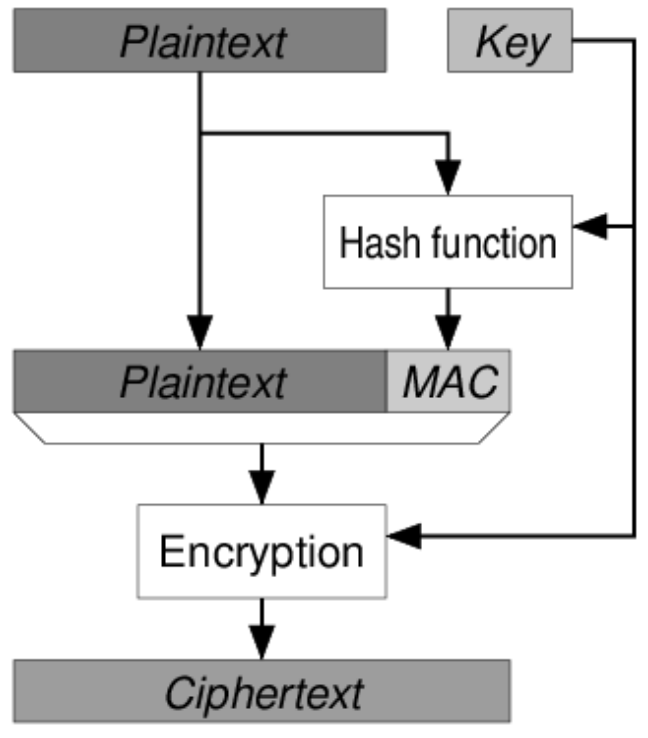
\includegraphics[width=0.8\linewidth]{figures/mte}
  \end{center}
\end{minipage}

\subsection{EtM - Encrypt than MAC}

\begin{minipage}{0.58\textwidth}
  Plaintext is first encrypted, then a MAC is produced based on the resulting ciphertext. 
  The ciphertext and its MAC are sent together.
  This combination reaches the higher security among the 4 approaches, if we assume that the MAC is strongly unforgeable.
\end{minipage}
\hfill
\begin{minipage}{0.38\textwidth}
  \begin{center}
    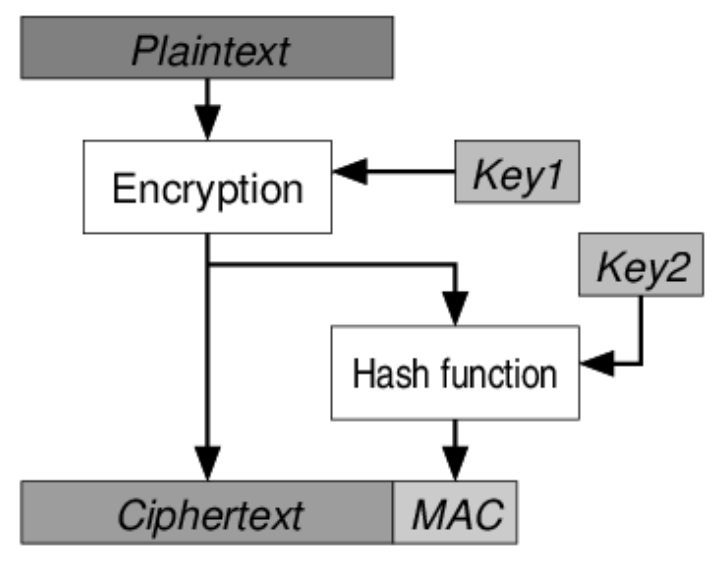
\includegraphics[width=0.85\linewidth]{figures/etm}
  \end{center}
\end{minipage}

\subsection{E\&M - Encrypt and MAC}

\begin{minipage}{0.58\textwidth}
  A MAC is produced based on the plaintext, and the plaintext is encrypted without the MAC.
  Are sent both the MAC and the encrypted data.
  This approach is used for example in SSH.
  E\&M has not yet been proved to be strongly unforgeable in itself, but some implementation can fix this.
\end{minipage}
\hfill
\begin{minipage}{0.38\textwidth}
  \begin{center}
    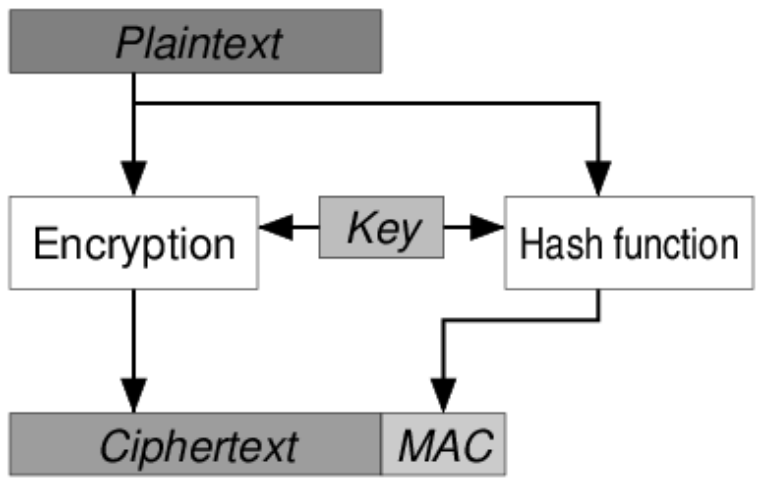
\includegraphics[width=0.85\linewidth]{figures/e&m}
  \end{center}
\end{minipage}

\section{Examples}

\subsection{CCM - Counter with Cipher block chaining Mac}

Was standardized by NIST specifically to support the security requirements of IEEE 802.11 WLANs\footnote{Wireless Local Area Networks} and is a variant of E\&M approach, which combines
\begin{itemize}
  \item AES: as the encryption cipher
  \item CTR: as the operation's mode
  \item CMAC: as the authentication algorithm
\end{itemize}
Is uses only one secret key, both for encryption and MAC.
\\\\
The mechanism of authentication and encryption of CCM are:
\begin{figure}[h]
  \begin{minipage}{0.48\textwidth}
    \begin{center}
      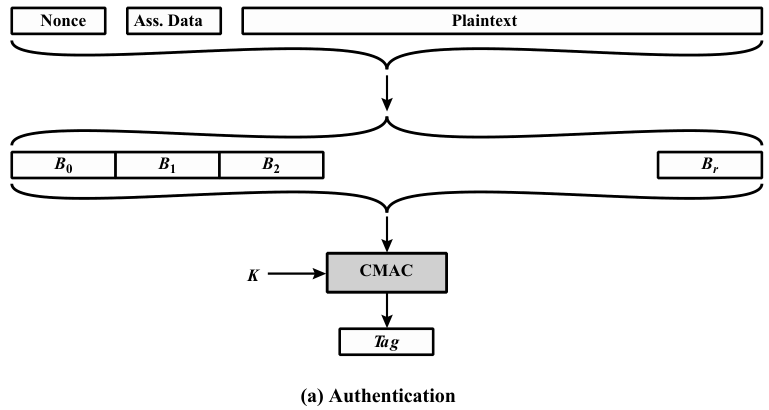
\includegraphics[width=\linewidth]{figures/ccm_auth}
    \end{center}
  \end{minipage}
  \hfill
  \begin{minipage}{0.48\textwidth}
    \begin{center}
      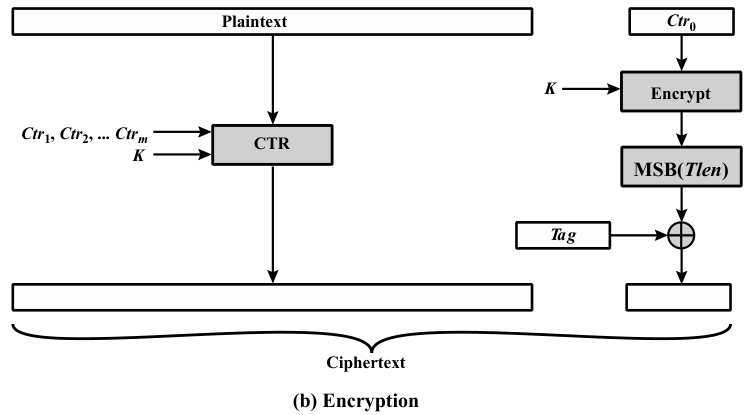
\includegraphics[width=\linewidth]{figures/ccm_enc}
    \end{center}
  \end{minipage}
\end{figure}

where the \textbf{associated data} is for example a protocol header and the \textbf{nonce} is a unique value that is different for every instance during the lifetime of a protocol association and is intended to prevent replay attacks and certain other types of attacks.

Associated data and nonce trivially need only authentication, while the real content data are both authenticated and encrypted.

\subsection{GCM - Galois Counter Mode}

The mechanism is the following:
\begin{itemize}
  \item the message is encrypted using a variant of CTR mode
  \item the resulting ciphertext is multiplied with a key over GF($2^{128}$)
\end{itemize}

\newpage

It uses the function \textbf{GHASH}, a keyed hash function, and \textbf{GCTR}, a variant of CTR using Galouis Fields.

Has been designed to be parallelizable so that it can provide high throughput with low cost and low latency, and is used for example in WPA3 and TLS.

\subsection{KW - Key Wrap}

It is an \textbf{operation mode} for securely exchange a symmetric key using another symmetric key (in this case called KEK) which was already shared by those parties.
It is very \textbf{slow}, but very \textbf{robust} because each bit of output can be expected to depend in a nontrivial fashion on each bit of input.

\section{PRNG - Pseudo Random Number Generator}

Use a \textbf{seed} value and a deterministic \textbf{algorithm} for generating a stream of pseudo-random bits.
The seed must be kept secret while the algorithm preferably not.
A hash function or MAC produces apparently random output and can be used to build a PRNG.
However, the problem is that with hash functions, the seed has a maximum length, thus sooner or later it must restart from the beginning, creating a \textbf{cycle}.
Equally, also MAC function can end in a cycle, because it can output different values and then after a certain point, it can generate an already previously generated value, entering a never ending cycle.
Both flaws are due to working over a \textbf{finite set of values}, thus sooner or later these values will finish and be reused in a way or another.

\chapter{Digital Signatures}

Digital signatures have been developed to \textbf{authenticate} messages' content, and to do so has been realized a verification function to check the signature of a message and in this way validate (or not) the contents, author and time of the message.
Signatures must be \textbf{verifiable by anyone}, and this is done using a public key.
A signature must depend on the message to sign, plus some more information that are known only to the sender to prevent both forgery and denial.
A signature must be \textbf{easy} to produce, store, distribute or verify, while being computationally \textbf{infeasible to forge}.

\section{Attacks}

For digital signatures there exists the following attacks:
\begin{itemize}
  \item \textbf{Key-only attack}: the attacker only knows victim's public key.
  \item \textbf{Known message attack}: the attacker has some messages and signatures.
  \item \textbf{Generic chosen message attack}: the attacker chooses the message to send, but he doesn't know the public key of the victim.
  \item \textbf{Directed chosen message attack}: the attacker chooses the message to send plus he knows the public key of the victim.
  \item \textbf{Adaptive chosen message attack}: the attacker chooses the message to send, also having a set of (message, signature) pairs of the victim.
\end{itemize}

\section{Forgery}

The possible message crafting scenarios for an attacker are:
\begin{itemize}
  \item \textbf{Existential forgery}: the attacker is able to force a signature over a message, but has no control over the message.
  \item \textbf{Selective forgery}: the attacker is able to force a signature over particular messages specifically crafted by the attacker.
  \item \textbf{Universal forgery}: the attacker finds an equivalent signing algorithm to craft equivalent signatures on arbitrary messages.
  \item \textbf{Total break}: the attacker determines the private key of the victim, thus can construct any (message, signature) pair he wants.
\end{itemize}

\section{Examples}

\subsection{Direct Digital Signature}

Is a digital signature schema that involves only the communicating parties, where the signature is computed using a private key over the hashed message (digest), then is sent with the plaintext.
The other party after having received the plaintext with the signature, can verify the authenticity by:
\begin{itemize}
  \item hashing the plaintext, \textit{i.e.} obtaining the digest
  \item compute the exponentiation of the signature that has received with the public key of the first party
  \item finally check if the computed digest matches the exponentiation output
\end{itemize}

The security of this schema depends on the \textbf{security} of the sender's \textbf{private key}.
In fact, if one of the two parties loses its private key, can declare it (revoke the key) and all the signatures produced with that key lose immediate validity.
This however leads to the possibility by the sender to deny, as he wishes, its own messages, \textit{i.e.} the schema is vulnerable to \textit{denial attacks}.
To overcome this problem has been added \textbf{timestamps} in the signature.

\subsection{ElGamal Digital Signature}

This signature schema copies asymmetric encryption mechanism, because works with two keys: one private, for signing, and one public, for verifying.
Each key pair is \textbf{user specific}, \textit{i.e.} each user has its own keys.
\\\\
ElGamal is composed of 4 phases:
\begin{enumerate}
  \item \textbf{parameter generation}
  \item \textbf{key generation}
  \item \textbf{signature}
  \item \textbf{verification}
\end{enumerate}

\subsubsection{1. Parameter Generation}

As first step are decided the following parameters:
\begin{itemize}
  \item key length $n$
  \item prime number $p$ of at least $n$ bits
  \item the hash function $H$
  \item a generator $g$, which is $<p$ and belongs the multiplicative group $Z_p^*$
\end{itemize}
then the pair $(p,g)$ is shared with the other parties (?).

\subsubsection{2. Key Generation}

Each user generates its key pair by:
\begin{itemize}
  \item choosing a \textbf{secret key} $x$ s.t. $1< x <p$
  \item computing the \textbf{public key} $y = g^x \bmod p$ 
\end{itemize}

The public key $y$ is also distributed to the other parties.

\subsubsection{3. Signature}

The signing mechanism is the following:
\begin{itemize}
  \item first is chosen an integer $k \in \left\{ 2, \ldots, p-2 \right\}$ coprime with the totient $p-1$.
  \item is computed $r = g^k \bmod p$
  \item is computed $s = \left( H(m) - xr \right) k^{-1} \bmod (p-1)$
\end{itemize}

The signature is the pair $(r,s)$ that must be sent along with the message.

\subsubsection{4. Verification}

The triple $(m,r,s)$ is valid iff it holds that
\begin{equation*}
  g^{H(m)} = y^r r^s \bmod p
\end{equation*}
and this means that $m$ has been really signed with $(r,s)$.

\subsection{DSA - Digital Signature Algorithm}

It is a variant of ElGamal and Schnorr schemas, built using SHA\footnote{Secure Hash Algorithm} as hashing function.
This solution has an approach similar to RSA, but added with \textbf{randomness}, in fact, if we sign the same message, with RSA we obtain the same output each time, while with DSA each output is different.

\begin{figure}[H]
  \centering
  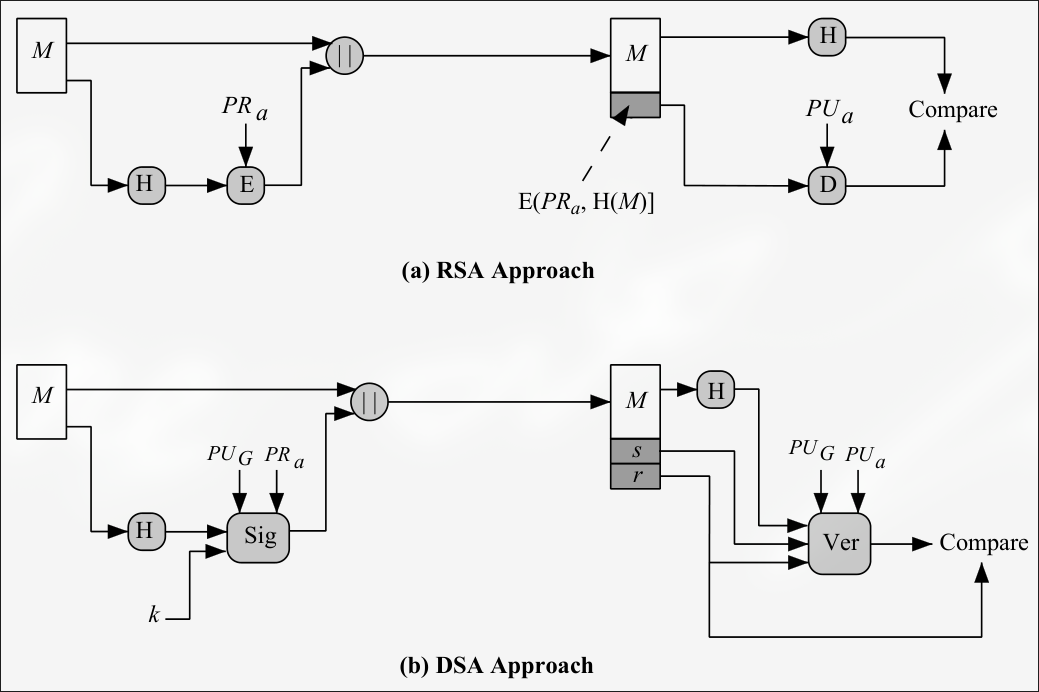
\includegraphics[width=0.6\linewidth]{figures/dsa_rsa_comparison}
\end{figure}

\subsubsection{Parameter setup}

Firstly are set up all the initial parameters
\begin{itemize}
  \item hash function $H$ (usually SHA-2)
  \item length $l > 2048$ bits
  \item modulus $n < l$
  \item $n$-bit prime $q$
  \item $l$-bit prime $p$, s.t. $p-1 \bmod q = 0$ (\textit{i.e.} $p-1$ is multiple of $q$)
  \item integer $h \in \left\{ 2, \ldots, p-2 \right\}$
\end{itemize}
From these parameters is then computed the generator $g = h^{\frac{p-1}{q}} \bmod p$.

With the global parameters $\left( p,q,g \right)$ each user can generate its key pair by firstly choosing a private key $x \in \left\{ 1, \ldots, q-1 \right\}$ and then computing the public one $y = g^x \bmod p$.

\subsubsection{Signature}

For signing a message $m$ is chosen a random temporary value $k \in \left\{ 1, \ldots, q-1 \right\}$ and then are computed:
\begin{itemize}
  \item $r = (g^k \bmod p) \bmod q$
  \item $s = k^{-1} \cdot \left( H(m) + xr \right) \bmod q$
\end{itemize}
The signature is the pair $\left( r,s \right)$.

\subsubsection{Verification}

To verify a signature $\left( r,s \right)$, one has to compute
\begin{itemize}
  \item $w = s^{-1} \bmod q$
  \item $u_1 = H(m) \cdot w \bmod q$
  \item $u_2 = r \cdot w \bmod q$
  \item $v = \left( g^{u_1}y^{u_2} \bmod p \right) \bmod q$
\end{itemize}
The signature is \textbf{valid} if we have $v = r$.

\subsubsection{Robustness}

The \textbf{entropy}, \textbf{secrecy} and \textbf{uniqueness} of $k$ are critical, otherwise an attacker is able to infer the private key $x$ of the signer.

\subsubsection{ECDSA}

There exists also a variant of DSA, called ECDSA\footnote{Elliptic Curve DSA}, which is implemented using Elliptic Curves, where all the participants of the digital signature scheme use the same global domain parameters, which define an elliptic curve and a point of origin on the curve.

\chapter{Cryptographic Key Management}

Cryptographic key management is the process of \textbf{administering} or \textbf{managing} cryptographic keys for a cryptographic system.
Furthermore, key management also involves the monitoring and recording of each key’s access, use and context.

\section{Key Distribution Techniques}

A successful key distribution implies delivering a key to two parties who wish to exchange data without allowing others to see or change the key.

\subsection{Symmetric Key Distribution}

The possible scenarios are
\begin{itemize}
  \item Alice generates a key and physically delivers it to Bob.
  \item a third party generates the key and physically delivers it both to Alice and Bob.
  \item if Alice and Bob have previously used a key, one of the two can use the now old key to encrypt the new key and deliver it.
  \item if Alice and Bob have a secure (encrypted) connection with a third party Charlie, then Charlie can generate the key and deliver it directly to both Alice and Bob.
\end{itemize}

\subsection{Symmetric Key Distribution using Asymmetric Keys}\label{sym_key_dist_with_asym_key}

Without using a third party the approaches are:
\begin{itemize}
  \item \textbf{simple plain send}:
    \begin{itemize}
      \item Alice sends its public key to Bob.
      \item Bob encrypts the symmetric key using the public key of Alice and sends it back.
    \end{itemize}
    This approach is \textbf{unsecure} not because the keys are in plain text, but because they can't assure the \textbf{authenticity} of the messages of each other.
    This distribution is unsecure against multiple attacks especially \textbf{MITM} attacks.
  \newpage
  \item \textbf{using nonce for challenge exchange}:
    \begin{itemize}
      \item Alice encrypts a nonce using the public key of Bob.
      \item Bob replies by sending the nonce of Alice concatenated with its nonce, all encrypted using the public key of Alice.
      \item Alice replies back by encrypting with the public key of Bob the nonce of Bob concatenated with the symmetric keys.
    \end{itemize}
    This approach is secure because of the \textbf{nonce} and by leveraging on the fact that only the owner of the asymmetric key pair is able to use his private key to decrypt the message and see the correct nonce of the other party to send back.
\end{itemize}
The second exchange is secure against MITM if and only if the public keys they have are correct, so in the next section we will see how to distribute public keys securely.

Using third party the approaches are:
\begin{figure}[H]
  \centering
  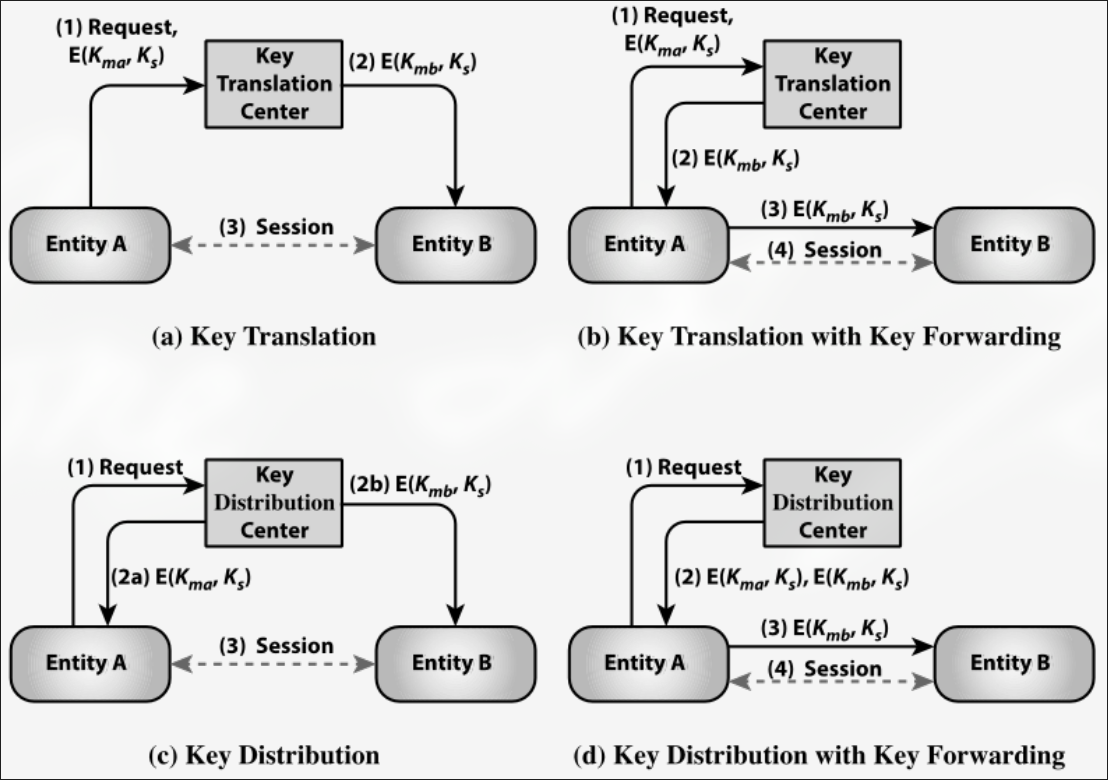
\includegraphics[width=0.7\linewidth]{figures/key_distribution}
  \caption{Symmetric key distribution using a third party and asymmetric keys}
\end{figure}
\subsection{Asymmetric Key Distribution}

\begin{enumerate}
  \item \textbf{Uncontrolled public key distribution}: the public key is just sent as it is to everyone in plaintext. This \textbf{isn't secure} for the same reason of the first example of symmetric key distribution with asymmetric keys~(section \ref{sym_key_dist_with_asym_key}). In fact this approach is prone to \textbf{replacement} attacks.
  \item \textbf{Public key Directory}: the mechanism is the same of the uncontrolled distribution with the minor difference that the public key isn't sent to everyone separately but to a key directory which stores the keys, and allows others to retrive the keys inside.
    This approach is for sure more efficient, but it's still unsecure.
  \newpage
  \item \textbf{Public key Authority}: use the same approach of public key directories, but the authority that manages the public keys, delivers the requested key by encrypting it with its private key.
    In this way the replacement attacks is not more feasible.
    A downside is that the PKA must be always online to complete the requests.
  \item \textbf{Certificate Authority}: further improvement of the public key Authority approach, because instead of storing and delivering public keys, the Certificate Authority, generates a certificate relative to the public key that has been sent. The party now has a certificate and can exchange it with other via a simple plain send to initialize a secure session with others.
\end{enumerate}

\begin{figure}[h]
  \begin{minipage}{0.48\textwidth}
    \centering
    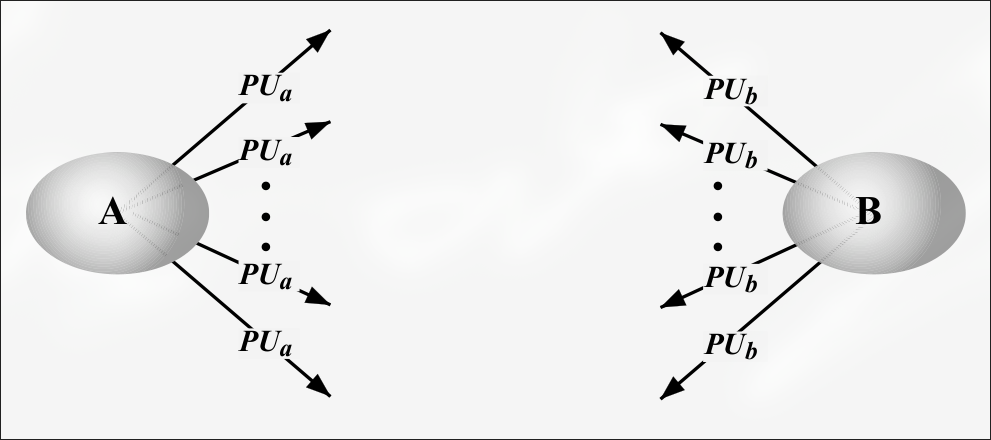
\includegraphics[width=\linewidth]{figures/uncontrolled_key_distribution}
    \caption*{1. Uncontrolled key distribution}
  \end{minipage}
  \hfill
  \begin{minipage}{0.48\textwidth}
    \centering
    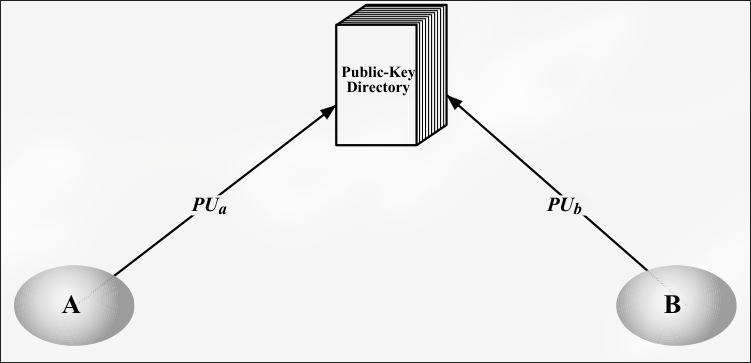
\includegraphics[width=0.93\linewidth]{figures/public_key_directory}
    \caption*{2. Public key Directory}
  \end{minipage}

  \vspace{20pt}
  \begin{minipage}{0.48\textwidth}
    \centering
    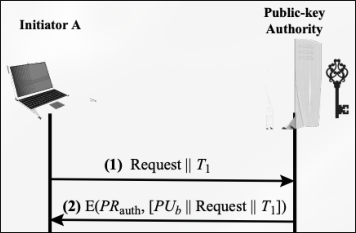
\includegraphics[width=0.8\linewidth]{figures/public_key_authority}
    \caption*{3. Public key Authority}
  \end{minipage}
  \hfill
  \begin{minipage}{0.48\textwidth}
    \centering
    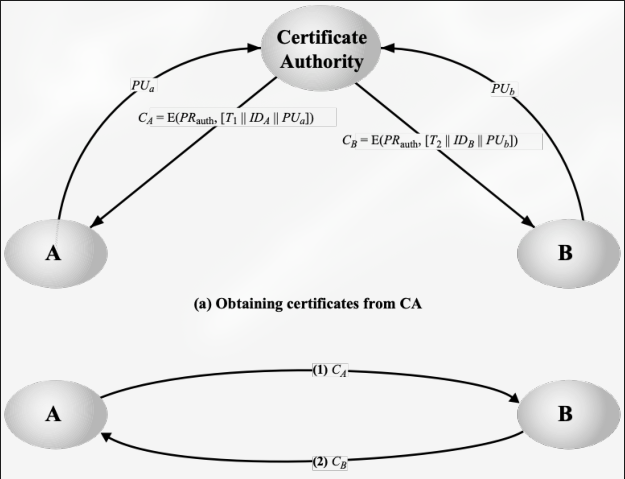
\includegraphics[width=\linewidth]{figures/certificate_authority}
    \caption*{4. Certificate Authority}
  \end{minipage}
\end{figure}

\section{Key Hierarchy}

\begin{itemize}
  \item \textbf{Master keys}: fewer, more robust but remain valid for a longer of time (even years).
  \item \textbf{Intermediate-level keys}: bigger quantity, can be reused but for a smaller amount of time than master keys (\textit{e.g.} session keys).
  \item \textbf{Ephemeral keys}: mainly are one-time keys, thus change at each use (\textit{e.g.} PGP, WhatsApp message encryption where each message has its own key).
\end{itemize}

\section{Certificates}

\textbf{X.509} is a certificate format for the provision to its users of authentication services by the \textbf{X.500 directory}, \textit{i.e.} the servers that maintain information about users.
Each certificate contains the public key of a user and is signed with the private key of a trusted certification authority.

The \textbf{extension} field specifies the \textbf{purposes} of requesting a certificate.
This is a crucial field added since version 3, because before everyone could use the fresh certificate to do everything he wanted, even use it to become a certificate authority itself.
This situation is avoided by specifying what can and can't be done with that certificate in the extension field.

By definition, certificates are \textbf{unforgeable}, thus can be stored without special protections.
In fact certificates generated by a CA have the following characteristics: 
\begin{itemize}
  \item Any user with access to the public key of the CA can verify the user public key that was certified.
  \item No party other than the certification authority can modify the certificate without this being detected.
\end{itemize}

Each certificate has a \textbf{period of validity}, however can be cases where the certificate must be updated before the expiration date, thus the current valid one is \textbf{revoked} and is produced a new one.
Some cases are:
\begin{itemize}
  \item the certificate owner loses its private key, or assumes it's been compromised
  \item the certification owner is no longer certified by the CA that released the certificate
\end{itemize}
For this reason, each CA must maintain a list of all revoked but not expired certificates issued by itself and this list should be posted in the directory (\textit{i.e.} publicly accessible).
\\\\
All these mechanisms and structures are joint together by the \textbf{Public Key Infrastructure}, which definition is a set of policies, servers and software which purpose is administering certificates.
The principal objective for developing a PKI is to enable secure, convenient and efficient acquisition of public keys.

%%%%%%%%%%%%%%%%%%%%%%%%%%%%
%%%%%%%%%%%%%%%%%%%%%%%%%%%%
%%%%%%%%%%%%%%%%%%%%%%%%%%%%
% SINCE THIS IS ALL CHECKED
%%%%%%%%%%%%%%%%%%%%%%%%%%%%
%%%%%%%%%%%%%%%%%%%%%%%%%%%%
%%%%%%%%%%%%%%%%%%%%%%%%%%%%

\section{Web of Trust}

In this scenario, the network and public key sharing process is based on \textbf{trust}.
Friends share keys with each other and each one trust the received keys because has been given by friends.
To expand the circle, one can receive an indirect trust from someone that is trusted by a friend of yours but not directly by you.
You can check his key with you friend and if valid you can trust it.
To sum this up, this exchange protocol is based on \textbf{direct exchanges} between parties and \textbf{indirect trust} through trusted parties.

This model can be extended adding a \textbf{degree of confidence}, \textit{i.e.} the more trusted parties certify a specific party's public key, the more that party can be trusted.

The difference with PKI is that PKI are built upon hierarchical centralized trust of CAs, while Web of Trust is \textbf{decentralized} and \textbf{without hierarchy}.
An example of Web of Trust is PGP\footnote{Pretty Good Privacy}.

\section{Quantum Key Distribution}

Quantum key distribution is a secure communication method enabling two parties to produce a shared random secret key known only to them, using a protocol based on quantum mechanics.
This is different from \textbf{quantum cryptography} which is used for encrypting, not sharing keys.
The key idea behind QKD is the strong assumption that passive attacks can't be perpetrated in quantum because seeing means measuring and this implies a modification of the data, thus the receiver is able to check if the message has been altered or not.

\subsection{BB84 protocol}

This protocol can be implemented only if two parties, Alice and Bob, are connected by a quantum communication channel and also a classical one.
Furthermore, any possible attacker can interact with both channels, however should not be able to modify the classical channel.
This protocol is based on \textbf{Heisenberg's Uncertainty principle} which state that in a quantum system, there exists a limit to the precision with which certain pairs of physical properties, such as position and momentum, can be simultaneously known. In other words, the more accurately one property is measured, the less accurately the other property can be known.

\subsubsection{Polarization of photons}

This protocol exploit Heisenberg's principle by applying it to the \textbf{polarization of photons}, mechanism needed to ``translate'' a photon to a classical bit in order to jump from a quantum channel to classical one.

The polarization of photons can be done over two different bases:
\\\\
\begin{minipage}{0.58\textwidth}
  \begin{itemize}
    \item the \textbf{rectilinear} basis: the photon is translated to 0 if is near the horizontal axis (H), otherwise if near the vertical one (V) is translated to 1.
    \item the \textbf{diagonal} basis: the photon is translated to 0 if is near the $45^\circ$ axis (D), otherwise if near the $135^\circ$ axis (A) is translated to 1.
  \end{itemize}
\end{minipage}
\hfill
\begin{minipage}{0.38\textwidth}
  \centering 
  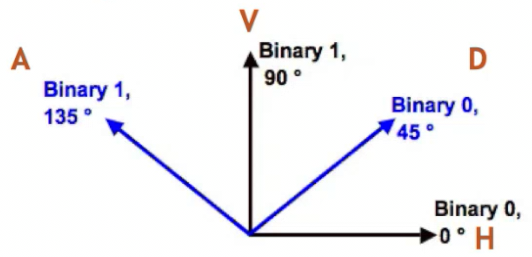
\includegraphics[width=\linewidth]{figures/photon_polarization_bases}
\end{minipage}

\subsubsection{Mechanism}

\begin{enumerate}
  \item Alice randomly selects a string of bits and a string of bases of equal length.
  \item She transmits a photon with the corresponding polarization for each bit on the quantum channel.
  \item Bob randomly chooses a basis for each photon received to measure its polarization, because he obviously cannot know in advance the bases chosen by Alice.
  \item Bob tells Alice what bases he used over the classical channel.
  \item Alice replies with the correctly guessed bases.
  \item Finally, they both remove the bits where Bob guessed incorrectly.
\end{enumerate}
The resulting string is the shared secret key.

\subsubsection{Robustness}

This protocol works even if we assume that there is an attacker that can inspect both channels (but not modify the classical one), because we combine the particular property of measurement in a quantum system along with probability.

In fact, an attacker Eve, to inspect the quantum bits, must:
\begin{itemize}
  \item intercept the qubits sent from Alice
  \item measure them to know their values
  \item decode them with guessed bases
  \item re-encode the bits in qubits 
  \item send these to Bob
\end{itemize}
Here comes the crucial point, Eve has $\displaystyle \frac{1 + \frac{1}{2} + \frac{1}{2} + 1}{4} = \frac{3}{4} = 75\%$ of probability over 1 qubit of guessing right the basis and transmit the qubit with no errors, \textit{i.e.} without being detected.
If Alice sends even only 20 qubits, this means that Eve probability of not introducing errors drops to $\left( \frac{3}{4} \right)^n = \left( \frac{3}{4} \right)^{20} = 0.003 = 0.3\%$, \textit{i.e.} has high chances of producing a high amount of errors in the received string by Bob.

All these errors can be easily detected because Bob has instead $\frac{3}{4}$ of probability of receiving the right qubit by guessing the basis, thus the amount of errors is way less and when comparing the basis with Alice, Bob can notice that there are too many wrong bits and that someone interfered with the message.
\\\\
However, this holds no more if the attacker Eve is also able to modify the classical channel data, because she can do a MITM attack, and be act like she's Bob with Alice and like she's Alice with Bob.

\chapter{User Authentication}

\begin{definition}[User Authentication]
  The process of determining whether some user, application or process, acting on behalf of a specific user, is really who or what it declares itself to be.
\end{definition}

Authentication is fundamental for \textbf{authorization}, which instead specifies what a user, application or process can/cannot do.
\\\\
We have also to distinct message authentication from entity authentication:
\begin{itemize}
  \item \textbf{Message} authentication: authenticates singular messages, one at a time, \textit{i.e.} each one has its own authentication.
  \item \textbf{Entity} authentication: authenticates a user for the entire duration of a \textbf{session}, thus each message sent by him is authenticated.
\end{itemize}

\section{Authentication Principles}

\begin{itemize}
  \item \textbf{Digital Identity} = is the unique representation of a subject in a digital environment.
  \item \textbf{Identity Proofing} = establishes that a subject is who they claim to be to a stated level of certitude.
  \item \textbf{Digital Authentication} = process of determining the validity of one or more authenticators used to claim a digital identity. It validates that the authenticated subject is in control of the technologies used to authenticate.
\end{itemize}

\section{Means of Authentication}

\begin{itemize}
  \item \textbf{Knowledge}: authentication by proving to know/remember a secret information (\textit{e.g.} password, PIN). The pros are that can be easily shared or updated, but on the contrary can be easy to guess.
  \item \textbf{Possession}: authentication by proving to be in control of a physical device (\textit{e.g.} OTP, hardware token, smart card). The pros are that cannot be cloned, but the cons are that are not so easily updatable and that can be lost.
  \item \textbf{Inherence}: authentication by proving some unique characteristics of an individual (\textit{e.g.} fingerprint, DNA, retina, face, voice, $\ldots$). These are not only biological, for example, using computer systems there are the serial numbers of the components, or can be used \textbf{PUF}\footnote{Physically Unclonable Functions}, which are small defected chips that generates almost unique outputs and are used for \textit{challenge-response} requests. The cons are the impossibility to be shared, lost or stolen and that are unforgeable, but on the cons are not updatable and can return false positive/negative (not everything so easy to trace).
\end{itemize}

These means of authentication can be used alone or can be combined.
In the second case, we call it a \textbf{multifactor/multi-layered} authentication.

\begin{note}
  Pay attention that using multiple authentications of the same type count as a single type and cannot be called multifactor authentication. To be called multifactor, someone must use \textit{different means} of authentication.
\end{note}

\section{Mutual Authentication Protocols}

Are protocols which allow communicating parties to \textbf{mutually check} each other’s \textbf{identity} and then enable the \textbf{session keys} exchange.
The two main problems of this protocol are:
\begin{itemize}
  \item \textbf{Timeliness}, which is an important factor to inhibit replay or MITM attacks.
  \item \textbf{Confidentiality}, because identification and session-key information must be communicated in encrypted form.
\end{itemize}

\subsection{Replay Attacks}

The main types of replay attacks are:
\begin{itemize}
  \item \textbf{simple replay}: message can be re-sent at any time in the future, \textit{i.e.} messages have no validity timeframe.
  \item \textbf{repetition that can be logged}: the same message is received twice within a valid timeframe.
  \item \textbf{repetition that cannot be detected}: occur if the receiver has deleted/lost the original message, thus cannot check if the message received is a repetition.
  \item \textbf{backward replay without modification}: the same message is sent back as it is to the sender.
\end{itemize}

Possible solution to cope with these attacks are:
\begin{itemize}
  \item attach a \textbf{sequence number} to each message, thus the receiver accepts the message only if the sequence value matches the expected one. Both parties must keep track of the last sequence value to be able to check the order of the messages received and their validity. Usually is not implemented because the value can be \textit{guessable} by the attacker with a minimum amount of tries and for the parties is pretty expensive to keep track of all the sequence numbers.
  \item implement a small \textbf{challenge-response} exchange with nonces to check the freshness of messages.
  \item add a \textbf{timestamp} to messages. Has the downsides that both parties must have a perfectly \textit{synchronized clock}, moreover the synchronization protocol sums up on the attack surface. Also is not easy to choose the \textit{validity interval} because we have also to consider the network speed traffic, \textit{i.e.} if the interval is too strict and the messages takes too much to be received, these are all discarded.
\end{itemize}

\subsection{Needham-Schr\"{o}der Private Key Protocol}

Is a third-party \textbf{key distribution protocol} for session between two parties $A$ and $B$, mediated by a trusted KDC\footnote{Key Distribution Center} and based on symmetric encryption.

The mechanism is the following:

\begin{minipage}{0.8\textwidth}
  \vspace{-10pt}
  \begin{align*}
    & 1. \quad A \rightarrow KDC: & & \left( ID_A \,\Vert\, ID_B \,\Vert\, R_A \right) \\
    & 2. \quad KDC \rightarrow A: & & \text{Enc}_{K_A} \left( K_S \,\Vert\, ID_B \,\Vert\, R_A \,\Vert\, \text{Enc}_{K_B} \left( K_S \,\Vert\, ID_A \right) \right) \\
    & 3. \quad A \rightarrow B: & & \text{Enc}_{K_B} \left( K_S \,\Vert\, ID_A \right) \\
    & 4. \quad B \rightarrow A: & & \text{Enc}_{K_S} \left( R_B \right) \\
    & 5. \quad A \rightarrow B: & & \text{Enc}_{K_S} \left( f(R_B) \right)
  \end{align*}
\end{minipage}

\vspace{10pt}
where
\begin{itemize}
  \item $ID$ is the user identifier
  \item $R$ stands for \textit{random number} and is used as a nonce
  \item $K_A$ and $K_B$ are the private keys of $A$ and $B$ respectively
  \item $K_S$ is the secret symmetric session key
  \item $f$ is a pre-defined function like $f(x) = x-1$
\end{itemize}

The first part of the protocol is a key exchange with the KDC to get a session key for $A$ and $B$, while the second part is a challenge-response exchange from $B$ to check the entity of $A$.
However, the step 3 is the most vulnerable because can be subject of replay attacks if an old session key has been compromised.
For this reason has been developed other variants such as the Denning-Sacco which adds a timestamp, and the Neuman which adds a nonce.

\subsection{Kerberos Protocol}

Kerberos provides a \textbf{centralized authentication} server whose function is to authenticate users to servers and vice versa, using only symmetric encryption.
The minimal requirements for Kerberos robustness are:
\begin{itemize}
  \item \textbf{security}: information must be secure against eavesdroppers.
  \item \textbf{reliability}: should implement a distributed architecture approach.
  \item \textbf{scalability}: the system must be able to support large numbers of clients and server.
  \item \textbf{transparency}: user should not be aware that authentication is taking place.
\end{itemize}
Kerberos was initially implemented using DES, then developers switched to AES.
\\\\
Kerberos' infrastructure is based on:
\begin{itemize}
  \item \textbf{Authentication Server}: stores all the users' passwords in a centralized database and shares a unique secret with each server.
  \item \textbf{Tickets}: it's returned by the AS after a user successful authentication from a server. A ticket is a file containing
    \vspace{-5pt}
    \begin{itemize}
      \item user ID
      \item network address
      \item server ID
    \end{itemize}
    which is encrypted using the \textit{Server-AuthenticationServer} shared secret.
  \item \textbf{TGS}\footnote{Ticket-Grating Server}: its job is to manage access requests for specific services by receiving the user ticket and generating a \textbf{service ticket}.
\end{itemize}
The client job is to store the user and service tickets, that will be used for authenticating the user to the server at each service access request.
Kerberos has been developed with the intention to be used in supervised small/medium environment like campuses or organizations and not publicly.
Kerberos version 5 has been developed to solve environmental and technical deficiencies of the version 4.

\section{Key Management}

\subsection{Via Public Key Encryption}

Public key encryption suits well the needs of session key distribution, however we need to be secure about the correctness of the other parties' keys.
The simplest, but still trusty, solution is to use an AS to distribute the public keys.

\subsubsection{Needham-Schr\"{o}der Public Key Protocol}

Even though exist also protocols based on nonces or timestamps, these are not used because have all being found flawed, for example the Needham-Schr\"{o}der Public Key Protocol (not to be confused with the private one seen previously).

\newpage

The protocol mechanism is the following:

\hspace{0.05\textwidth}
\begin{minipage}{0.95\textwidth}
  \vspace{-5pt}
  \begin{align*}
    & 1. \quad A \rightarrow AS: & & \left( ID_A \,\Vert\, ID_B \right) & & \text{$A$ asks the $AS$ for $B$ public key.} \\
    & 2. \quad AS \rightarrow A: & & \text{Enc}_{PR_{AS}} \left( PU_B \,\Vert\, ID_B \right) & & \text{The $AS$ responds by signing the public key of $B$ with} \\ & & & & & \text{its private key to protect the message from alteration.} \\
    & 3. \quad A \rightarrow B: & & \text{Enc}_{PU_B} \left( N_1 \,\Vert\, ID_A \right) & & \text{$A$ challenges $B$ by encrypting a nonce $N_1$ with $B$} \\ & & & & & \text{public key.} \\
    & 4. \quad B \rightarrow AS: & & \left( ID_B \,\Vert\, ID_A \right)  & & \text{$B$ does the same first step of $A$.} \\
    & 5. \quad AS \rightarrow B: & & \text{Enc}_{PR_{AS}} \left( PU_A \,\Vert\, ID_A \right) & & \\
    & 6. \quad B \rightarrow A: & & \text{Enc}_{PU_A} \left( N_1 \,\Vert\, N_2 \right) & & \text{Only $B$ is able to decrypt the message from $A$ and to} \\ & & & & & \text{get the nonce $N_1$, thus responds proposing the same} \\ & & & & & \text{challenge to $A$.} \\
    & 7. \quad A \rightarrow B: & & \text{Enc}_{PU_B} \left( N_2 \right) & & \text{$A$ confirms the challenge by replying with just} \\ & & & & & \text{the nonce $N_2$.}
  \end{align*}
\end{minipage}

\vspace{10pt}
where $AS$ is the Authentication Server and $N_1, N_2$ are two nonces used for challenge-response between $A$ and $B$.
\\\\
Even though it seems a secure protocol, has been shown with a static model checker that instead it is vulnerable against \textbf{Lowe's attack}, which is a MITM by an attacker C, who doesn't alter the traffic to and from the AS, but only manipulates the packets between A and B, in the following way:

\hspace{0.05\textwidth}
\begin{minipage}{0.95\textwidth}
  \vspace{-5pt}
  \begin{align*}
    & 3A. \quad A \rightarrow C: & & \text{Enc}_{PU_C} \left( N_1 \,\Vert\, ID_A \right) & & \text{$A$ is trying to initialize a clean session with $C$.} \\
    & 3B. \quad C \rightarrow B: & & \text{Enc}_{PU_B} \left( N_1 \,\Vert\, ID_A \right) & & \text{$C$ relays the message to $B$ pretending to be $A$} \\ & & & & & \text{and to be initializing the session exchange with him.} \\
    & 4. / 5. & & & & \text{The messages between $B$ and the $AS$ are left untouched.} \\
    & 6. \ \ \quad B \rightarrow A: & & \text{Enc}_{PU_A} \left( N_1 \,\Vert\, N_2 \right) & & \text{$B$ can respond directly to $A$, because $C$ already} \\ & & & & & \text{knows $N_1$, thus it doesn't intervene.} \\
    & 7A. \quad A \rightarrow C: & & \text{Enc}_{PU_C} \left( N_2 \right) & & \text{$A$ receiving back its nonce $N_1$ assumes it can only} \\ & & & & & \text{be the response from $C$, so she responds back with} \\ & & & & & \text{the nonce $N_2$.} \\
    & 7B. \quad C \rightarrow B: & & \text{Enc}_{PU_B} \left( N_2 \right) & & \text{$C$ decrypts $A$'s message and re-encrypts it for $B$.}
  \end{align*}
\end{minipage}

\vspace{5pt}
\begin{note}
  The message order is kept the same of the real protocol mechanism
\end{note}

\vspace{5pt}
The connection is now established and $B$ thinks to be talking to $A$ and that only he and $A$ know the nonces $N_1, N_2$.

\newpage

A variant almost identical is the following, but with the difference that also $A$ is being tricked by $C$ and this is a both ways MITM:

\hspace{0.05\textwidth}
\begin{minipage}{0.95\textwidth}
  \vspace{-5pt}
  \begin{align*}
    & 1. \ \ \quad A \rightarrow AS: & & \left( ID_A \,\Vert\, ID_B \right) & & \text{$C$ only intercepts the message, so the $AS$ will not} \\ & & & & & \text{respond.} \\
    & 1B. \quad C \rightarrow AS: & & \left( ID_A \,\Vert\, ID_C \right) & & \text{$C$ makes a request to the $AS$ by behaving as $A$.}\\
    & 2. \ \ \quad AS \rightarrow A: & & \text{Enc}_{PR_{AS}} \left( PU_C \,\Vert\, ID_C \right) & & \text{This step remains the same.} \\
    & 3A. \quad A \rightarrow C: & & \text{Enc}_{PU_C} \left( N_1 \,\Vert\, ID_A \right) & & \text{$A$ thinks to be talking to $B$ and sends the challenge} \\ & & & & & \text{to $C$.}
  \end{align*}
\end{minipage}

\vspace{15pt}
The remaining steps are the same.
\\\\
A simple \textbf{patch} that fixes both variants is to include $ID_B$ in the first nonce response from $B$, \textit{i.e.} the message becomes $\text{Enc}_{PU_A} \left( N_1 \,\Vert\, N_2 \,\Vert\, ID_B \right)$.

\section{ProVerif}

Authentication protocols are very difficult to be proved correct, thus is a must to use \textbf{formal methods} (ProVerif, Tamarin) to assess their real security.
\\\\
For example, ProVerif is an automatic (\textit{i.e.} not interactive) symbolic verifier for cryptographic protocols, based on \textbf{Horn clauses}, which are disjunctions of literals ($f_1 \land f_2 \land \ldots \land f_n$) where \textbf{at most} one of them is True.
It takes as \textbf{input} an abstraction of the protocol, plus some security queries among the following types:
\begin{itemize}
  \item \textbf{Secrecy}: defines a message as secret from attackers.
  \item \textbf{Correspondence}: guarantees that a message has really been sent by the sender.
  \item \textbf{Equivalence}
\end{itemize}

The entire input is converted to Horn clauses before being given to the algorithm.

The algorithm output tells if the protocol is vulnerable, \textit{i.e.} if there is a possible attack.

\section{One-Way Authentication}

In some scenarios, it can happen that we want to be able to authenticate two parties even though messages can go only in one way, \textit{e.g.} $Alice$ can send messages to $Bob$, but not vice versa, but we still want $Bob$ to be able, for example, to authenticate $Alice$.
\textbf{Emails} are the most famous example of one-way communication, because each message ends with itself, there is no need for a reply, \textit{i.e.} there can be, but is not needed for the communication itself to work.


\newpage

There are several approaches depending on the aim:
\begin{itemize}
  \item \textbf{Confidentiality}:
    \begin{equation*}
      A \rightarrow B: \text{Enc}_{PU_B}(k), \text{Enc}_k(M)
    \end{equation*}
    In this way $Bob$ is the only one able to get $k$ and decrypt $M$.
    Even though it may seem odd, encrypting directly the message with the public-key of $Bob$ is inefficient in the long run, because $k$ is smaller than $M$ and asymmetric encryption is way slower than symmetric one, furthermore once $Bob$ has $k$, the following messages can all be encrypted with $k$.
    However, this solution falls short in proving authentication by Alice.
  \item \textbf{Authentication}: to provide authenticity about a message $M$, $Alice$ can send:
    \begin{equation*}
      A \rightarrow B: M, \text{Enc}_{PR_A}(H(M))
    \end{equation*}
    This proves that only $Alice$ can have sent the message $M$, thus she cannot later deny it.
    By sending the hash, $Alice$ guarantees also the integrity of $M$.

    However, this is vulnerable to replay attacks because there is nothing that guarantees freshness, which can be solved, for example, by concatenating a timestamp $T$ to the hash.
    Obviously, because we are talking about one-way communications, nonces are useless for proving freshness because we cannot implement a challenge-response mechanism.
  \item \textbf{Confidentiality AND Authentication}: we can combine the two messages above to guarantee both properties:
    \begin{equation*}
      A \rightarrow B: \text{Enc}_{PU_B}(k), \text{Enc}_k(M, \text{Enc}_{PR_A}(H(M)))
    \end{equation*}
    This schema is largely adopted in mail security (PGP, S/MIME).
\end{itemize}

\section{Federated Identity Management}

Is born as a solution to the increasing number of digital services, which implies an identity (user + password) for each of them.
The FIM proposes the use of a \textbf{unique verified identity} to authenticate over multiple enterprises and applications.

The identity management is \textbf{centralized} and \textbf{automated}, allowing any authorized individual, \textit{e.g.} employees, to access the services they need.
This concept of single identity relies on another new security mechanism which is the \textbf{Single Sign-On}, which enables a user to access all network resources after a single authentication.

To be \textbf{GDPR compliant} the identity provider should use only the data of a user that, without even one of them, it cannot verify correctly the identity.
For example a cigarettes vending machine should only need to check a single boolean attribute value (True/False) that tells if the user is over 18 or not, while a NON GDPR compliant machine can read all the information on the card and if its malicious is can also store these data.

\section{OAuth2}

It is an alternative to FIM, where the services don't belong to the same organization, but are provided by \textbf{different} and \textbf{independent} ones.
In this way, a user is able to log in an application without the need of a specific account for it, but instead using the account of another app that already have.

In fact, OAuth2 is an authorization mechanism that allows websites to request \textbf{restricted access} to another application’s account.
The other application can authorize the access without revealing the login credential with the website, but by sharing an \textbf{access token} via OAuth2.
For example, the website Doodle provides the possibility to login via OAuth2 using a Google account.
\\\\
The mechanism is based on the following parties:
\begin{itemize}
  \item \textbf{Client application}: the website/application requesting access (\textit{e.g.} Doodle).
  \item \textbf{OAuth service provider}: is like the identity provider, and its job is to process, manage and check user's data (\textit{e.g.} accounts.google.com).
  \item \textbf{Resource owner}: application that own the data, \textit{i.e.} where are stored the data (\textit{e.g.} Google Calendar).
\end{itemize}

OAuth2 has 4 different variants called \textbf{flows}:
\begin{itemize}
  \item \textbf{Authorization code grant}: after the user logs in the authorization server, is redirected to the client application via a redirection URL that contains a code. This code is extracted by the client application and exchanged with the authorization server to obtain the final access token. Is the most used and is used also in the example above.
  \item \textbf{Implicit grant}: after the user logs in the access token is returned directly. It is deprecated in favor of the previous type, because lacks the additional exchange step which is used as a confirmation that the client has received the code.
  \item \textbf{Client credential grant}: the access token authenticates the client not the user. It's typically used by clients to access resources about themselves rather than to access a user's resources. There is no user interaction because the application executes the authentication request directly for itself.
  \item \textbf{Password grant}: is another legacy type like the implicit grant, which is not recommended to use. The user provides the login information (\textit{e.g.} username and password) to the client application, which sends them directly to the authorization server to receive the token. The user must \textbf{fully trust} the client application in order to give it its credentials.
\end{itemize}

\chapter{TLS - Transport Level Security}

Web servers need \textbf{tailored security} tools to avoid being exploited and used as a bridge to get into the backend servers of the corporations, which are usually full of security flaws because of their inner complexity.

\textbf{SSL}\footnote{Secure Socket Layer} and \textbf{TLS}\footnote{Transport Layer Security} work over TCP and offer \textbf{integrity} and \textbf{confidentiality}.
Building a new protocol would have implied replacing the current used ones and this comes with big costs, thus SSL has been designed to be an intermediate additional layer with the minimum differences possible in the way sockets were used until then, to allow a \textbf{smooth adoption} process.
In fact, most of the calls are similar to sockets, however has some own specific calls.
TLS is nothing more than a new standard that has simply replaced SSL.

Updating a protocol from an organization point of view, means \textbf{porting} each service on the new protocol version, \textit{i.e.} merging all the differences that have been introduced with the update.
It's not difficult because it only requires to \textbf{access} and \textbf{modify} the \textbf{source code} of your services, however can be tedious if a lot of methods and parameters values has changed and need to be fixed.
Sometimes can even cause problems, for example if the source code has been lost or if the developer has gone away.

\section{Architecture}

TLS is composed by two layers:
\begin{enumerate}
  \item \textbf{Record Protocol}: implements the actual \textbf{security transformation} of data from/to the TCP insecure channel, in fact uses \textbf{TCP sockets} for data transmission.
    Is used directly by applicative protocols like HTTP or IMAP and belongs to \textbf{layer 6} of the ISO/OSI stack, \textit{i.e.} presentation layer.
    To work needs to use information kept in the \textbf{connection state}, which are managed by the other protocols.
  \item \textbf{Handshake, Cipher Change and Alert Protocols}: are used for entity authentication to set up and manage the information needed by the security services, but also for handling possible connection errors.
    These belong to the \textbf{layer 5}, \textit{i.e.} session layer.
\end{enumerate}

\vspace{5pt}

\begin{figure}[h]
  \begin{center}
    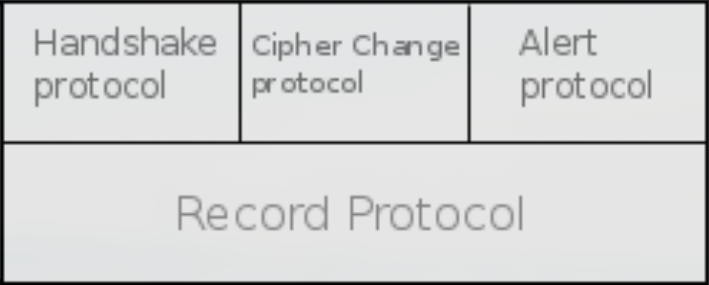
\includegraphics[width=0.35\linewidth]{figures/TLS_layers}
  \end{center}
\end{figure}

\newpage

In TLS we distinguish between:
\begin{itemize}
  \item \textbf{Session}: needed to \textbf{associate client and server}, it's initialized by the Handshake protocol by setting up all the \textbf{security parameters} in the session state:
    \vspace{-5pt}
    \begin{itemize}
      \item \textit{Session identifier} of 8 bits
      \item \textit{Peer certificate}
      \item \textit{Compression method}
      \item \textit{Cipher specs}: there are several choices for each aspect (Key exchange, Data Encryption Cipher, Authentication and Message Authentication), yielding more than 300 different specifications, called \textit{suites}. Each possible suite has its own string identifier (\textit{e.g.} \texttt{TLS\_ECDHE\_RSA\_WITH\_AES\_128\_CBC\_SHA256}).
      \item \textit{Master secret}: 48-bytes shared key
    \end{itemize}
    \vspace{-5pt}
    Once the session is established, it's used for all the following connections.
  \item \textbf{Connection}: is an \textbf{ephemeral communication} link associated to a session, where happens the real data flow.
    Each connection has its own parameters stored in the connection state, which are:
    \vspace{-5pt}
    \begin{itemize}
      \item Two \textit{random numbers}, one for the server and the other for the client
      \item A set of 6 different \textit{secrets} which are derived from the master secret
      \item A \textit{sequence number} in [0, $2^{64} - 1$]
    \end{itemize}
    \vspace{-5pt}
\end{itemize}

\begin{figure}[h]
  \begin{center}
    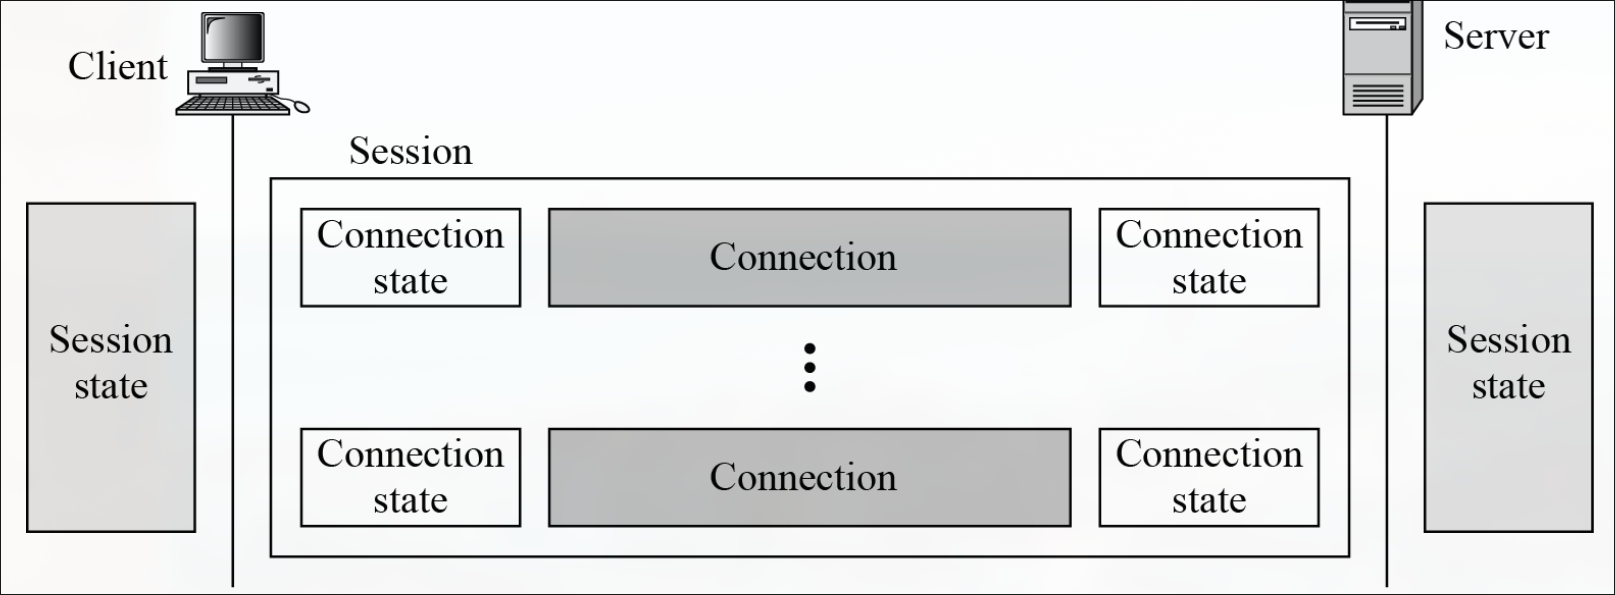
\includegraphics[width=0.7\linewidth]{figures/session_vs_connection}
  \end{center}
\end{figure}

\section{Handshake Protocol}

It establishes the session data and does this in 4 phases:
\begin{enumerate}
  \item The client proposes its \textbf{choice of parameters} (TLS version, list of cipher suite available, compression method and the random numbers) to the server, who can agree responding with a confirmation of the parameters. For the cipher suite, the server chooses the first that matches its list, thus if there is no suite accepted both by client and server, then the server declines the connection.
  \item In this phase, the server may send a list of certificates, its public key and request a certificate, then it sends the ``\textit{Server Hello}'' and the \textbf{server is authenticated} for the client.
  \item The client may reply to the optional certificate request by sending its list of certificates, its public key and the hash of the certificates (to prove their integrity). Obviously, if the server never requested a certificate, the client doesn't send anything and it simply becomes authenticated for the server. The \textit{pre-master} key is computed from the keys exchanged or from the certificates' data, depending on the data exchanged in phase 2 and 3.
  \item Cipher specs and hashes are exchanged by both parties.
\end{enumerate}
At the end of these 4 phases, client and server are ready for exchanging data.
\\\\
Four common examples of phases 2 and 3:

\vspace{-5pt}
\begin{figure}[h]
  \begin{minipage}{0.48\textwidth}
    \centering
    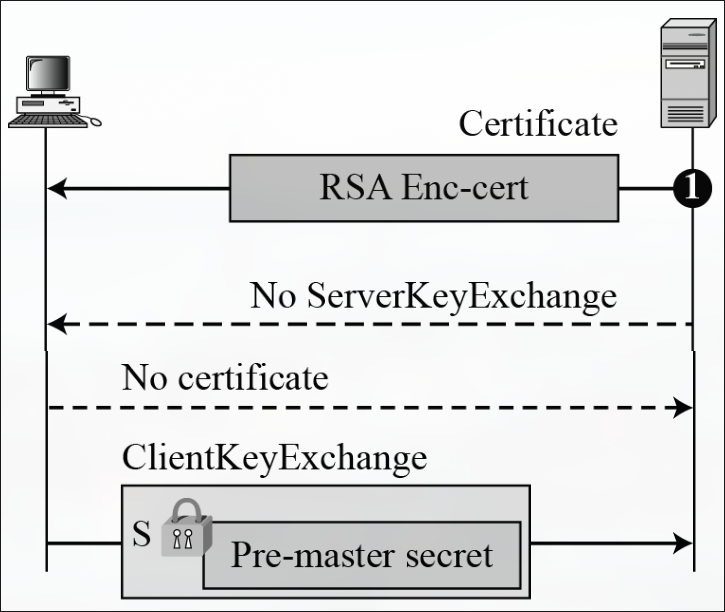
\includegraphics[width=0.8\linewidth]{figures/handshake_rsa}
    \caption*{(1) RSA}
  \end{minipage}
  \hfill
  \begin{minipage}{0.48\textwidth}
    \centering
    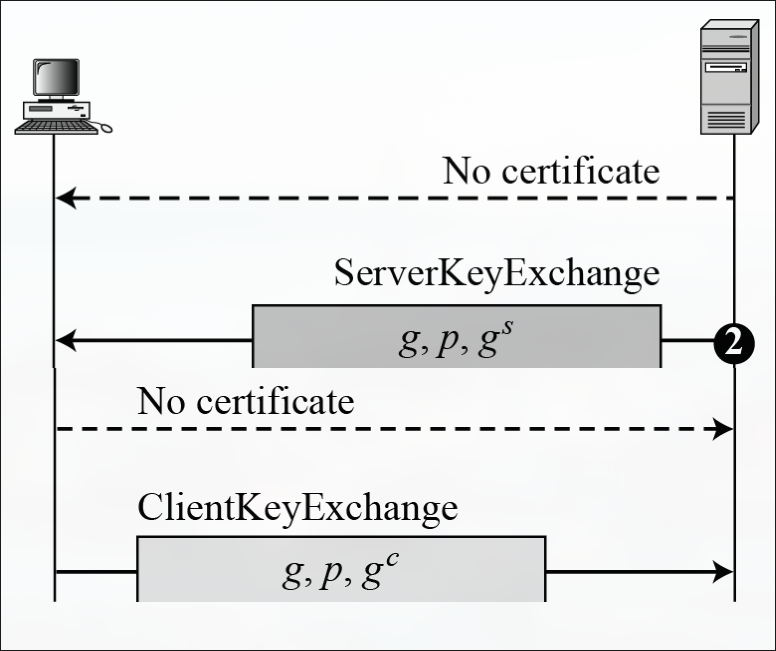
\includegraphics[width=0.8\linewidth]{figures/handshake_dh_anonymous}
    \caption*{(2) Anonymous DH}
  \end{minipage}
  
  \begin{minipage}{0.48\textwidth}
    \centering
    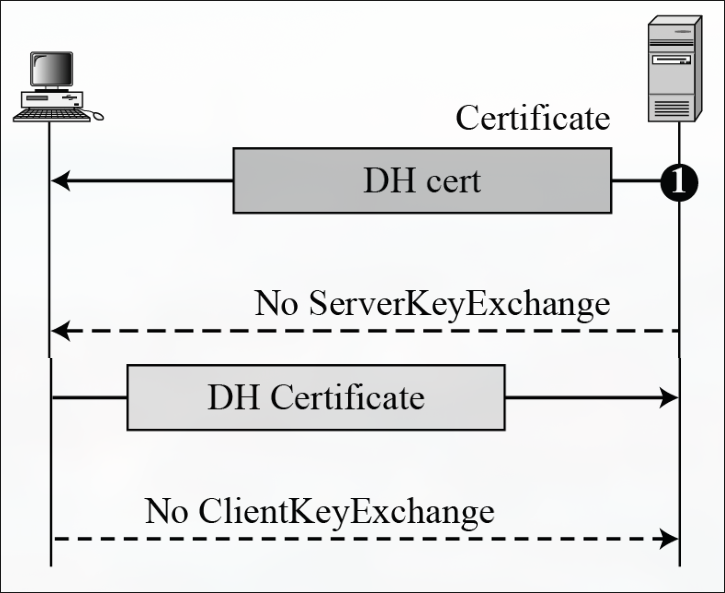
\includegraphics[width=0.85\linewidth]{figures/handshake_dh_fixed}
    \caption*{(3) Fixed DH}
  \end{minipage}
  \hfill
  \begin{minipage}{0.48\textwidth}
    \centering
    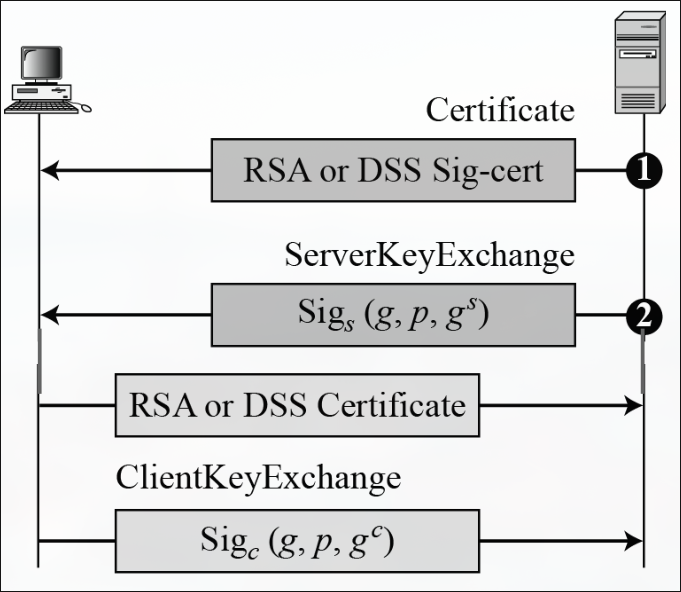
\includegraphics[width=0.8\linewidth]{figures/handshake_dh_ephemeral}
    \caption*{(4) Epheremeral DH}
  \end{minipage}
\end{figure}

\vspace{-10pt}
\begin{enumerate}
  \item With RSA, only the server is authenticated for the client (no true vice versa) and this is the most common scenario.
  \item Anonymous DH, \textit{i.e.} DH with no authentication, is vulnerable against MITM attacks due to the anonymity.
  \item In fixed DH, the public data are available in the certificate. However, because the certificate isn't refreshed often, the derived pre-master key remains the same, even between different sessions. 
  \item Ephemeral DH is the most robust and is the recommended choice if possible. Requires that both client and server have a X.509 certificate. Is DH using the client and server random numbers for the key exchange, plus everything is signed with RSA (or DSS).
\end{enumerate}

The master key is computed combining the pre-master key and the client and server random values via a \textbf{pseudo-random function} derived from HMAC.

\section{Connection State}

After the session is established, one or more connections can be made and, for each of them, are used different \textbf{secrets} and \textbf{IVs}.
The 6 secrets (48 bytes / 8 bytes = 6 different keys) are derived from the session master key, which is stored in the session state, using the same algorithm used for generating the master key.

\begin{figure}[h]
  \begin{center}
    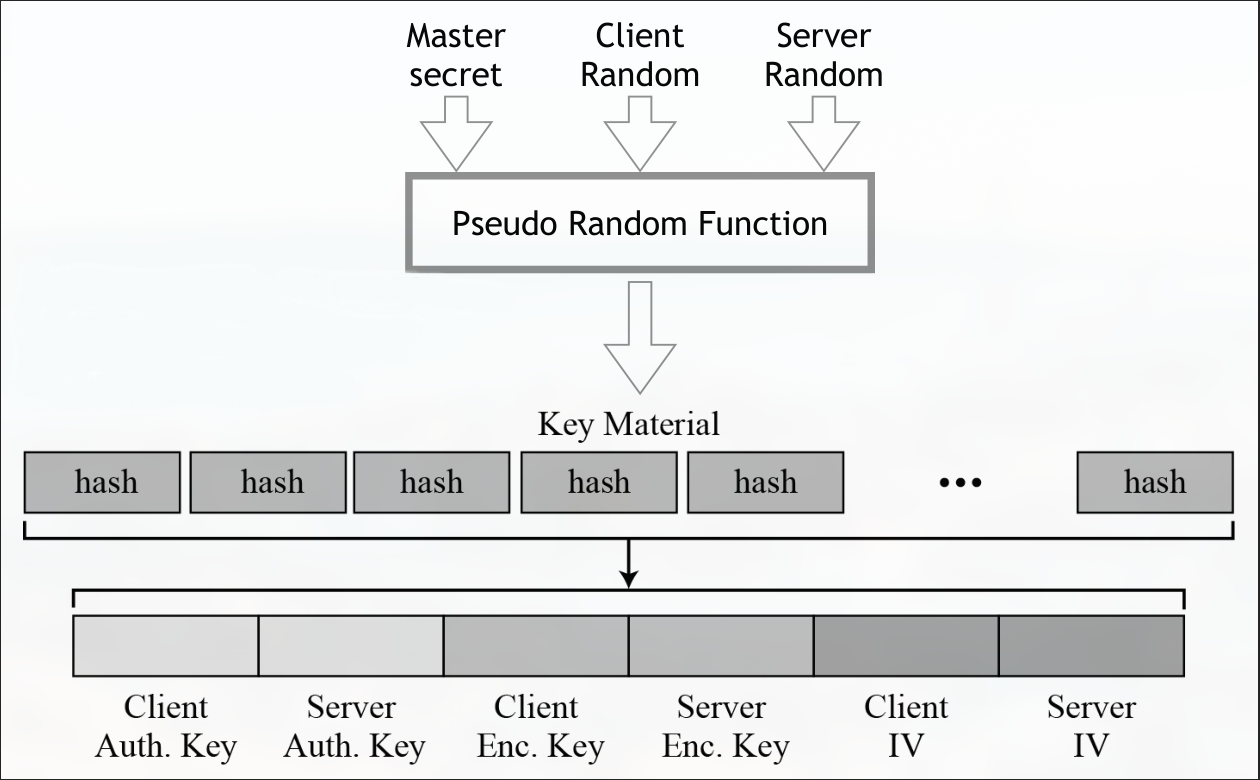
\includegraphics[width=0.7\linewidth]{figures/connection_secrets_gen}
  \end{center}
\end{figure}

\section{Record Protocol}

\begin{minipage}{0.48\textwidth}
  In this protocol are implemented the security transformations, using the parameters of the connection.

  Each message is also \textbf{fragmented and compressed}, before being transformed by security functions.

  For the \textbf{integrity} is used a MAC with the shared key, while for \textbf{confidentiality} is used symmetric encryption.
  For the calculation of the MAC is also used the sequence number (but not sent) to avoid replay attacks.

\end{minipage}
\hfill
\begin{minipage}{0.48\textwidth}
  \centering
  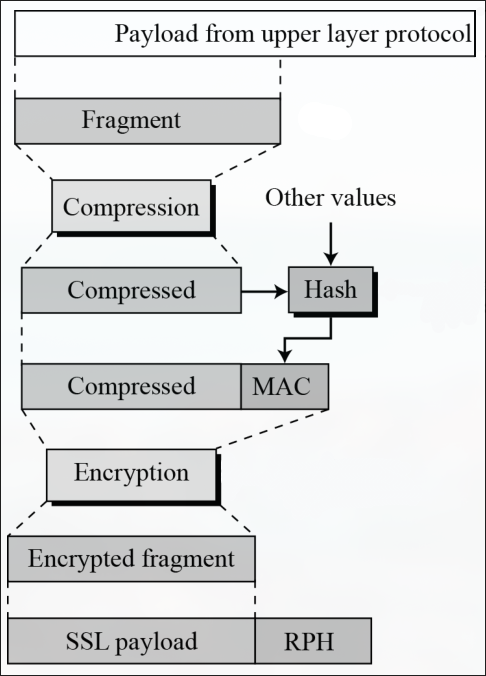
\includegraphics[width=0.7\linewidth]{figures/record_protocol}
\end{minipage}

\section{TLS 1.3}

Currently, it's the latest version available and with the previous version many aspects have changed and have been simplified.
The most notable differences are:
\begin{itemize}
  \item Encryption and authentication have been replaced with a combined version called AEAD\footnote{Authenticated Encryption with Associated Data}.
  \item In the HMAC key derivation function (HKDF), it must also be used an hash algorithm.
  \item Ciphers must use an \textit{ephemeral key exchange} algorithm so that new key pairs are generated for every exchange 
  \item The handshake protocol has been reduced from two to only one exchange for 
\end{itemize}
Furthermore, there have been removed also some cipher specs like:
\begin{itemize}
  \item Key exchange: RSA
  \item Encryption: RC4, DES, 3DES
  \item Cryptographic hash algorithms: MD5, SHA-1 
  \item Cipher Modes: AES-CBC  
\end{itemize}
but also many other features not listed here. Having reduced the available cryptographic choices, TLS 1.3 supports only 5 suites, which are:
\begin{itemize}
  \item \texttt{TLS\_AES\_128\_GCM\_SHA256}
  \item \texttt{TLS\_AES\_256\_GCM\_SHA384}
  \item \texttt{TLS\_CHACHA20\_POLY1305\_SHA256}
  \item \texttt{TLS\_AES\_128\_CCM\_SHA256}
  \item \texttt{TLS\_AES\_128\_CCM\_8\_SHA256}
\end{itemize}
following the security concept of ``less is more''.

The string identifier is read in the following way:
\begin{align*}
  \text{TLS} \quad & \_ \quad \text{AES\_128\_GCM} \quad \_ \quad \text{SHA256} \\
  \text{Protocol} \quad & \_ \quad \ \text{AEAD cipher} \quad \ \_ \quad \text{HKDF hash algorithm}
\end{align*}

\section{Attacks}

We can categorize the possible attacks against SSL/TLS in:
\begin{enumerate}
  \item against the handshake
  \item against the record and application protocols
  \item against the PKI\footnote{Public Key Infrastructure}: \textit{e.g.} try to change the certificates used
  \item other attacks
\end{enumerate}

\section{HTTPS}

HTTP have to be aware of the underlying protocols, for example, have to take into account if is using TLS or not, otherwise an attacker can trick HTTP to try change keys or avoid using TLS.

Initialization/Closure request have to flow from HTTP, then TLS and finally TCP following the TCP/IP structure.
For example, when closing an HTTP connection, HTTP has to tell TLS to start the session closing process, and can't be otherwise, because TLS cannot read HTTP traffic and also the closing alert has to be communicated before having closed the connection, otherwise an unannounced closure could be exploited for some attacks.
Opening order must happen downward, while closing order must happen upward.

\section{SSH}

Has been implemented to be a secure/encrypted version of Telnet, \textit{i.e.} for a simple and inexpensive remote access.
SSH stack structure is similar to TLS.

\chapter{Wireless Network Security}

Wireless are more vulnerable to attacks than wired one, because the traffic have to flow freely in the air, so it can be captured and eavesdropped.
Is also more inefficient, stable and less performant than a wired connection, and this leads wireless network to be more vulnerable to jamming.
Wireless networks on the other hand are mobile, but this comes with increased risks.

\section{Threats}

\begin{itemize}
  \item \textbf{Accidental association}: LANs in close proximity, may create a \textbf{transmission overlap}, such that a user intending to connect, may accidentally end connected with the \textbf{wrong access point}.
  \item \textbf{Malicious association}: a wireless device is set up in such a way that \textbf{seems} another \textbf{legitimate} access point, but instead has malicious intentions, like stealing credentials for the legitimate counterpart, for example by setting the same SSID of another access point and logging all the password attempts.
  \item \textbf{Ad-hoc network}: like peer-to-peer networks without an access point in between. A lack of a central point of control may become a  security risk.
  \item \textbf{Non-traditional networks}: like bluetooth, barcodes or PDAs, which are an additional risk in terms of eavesdropping and spoofing.
\end{itemize}

\section{Attacks}

\begin{itemize}
  \item \textbf{Identity theft}: also called \textbf{MAC spoofing}, occurs when an attacker is able to identify the MAC address of a connected computer, by eavesdropping on a network traffic.
  \item \textbf{MITM}: emulates a direct connection between a user and an access point, while the attacker stand in the middle and works like a relay. Wireless networks are very vulnerable against this attack.
  \item \textbf{DoS}: access points are very vulnerable because have limited resources and can easily be ``filled up'', leading to unexpected behaviors or becoming unusable for the network users.
  \item \textbf{Network injection}: this attacks specifically access points that manage unfiltered network traffic, \textit{e.g.} routing protocols or network management.
\end{itemize}

\section{Security}

In general, to secure a wireless network, we want to avoid
\begin{enumerate}
  \item eavesdropping
  \item unauthorized access
  \item alteration/insertion of messages
  \item disruption
\end{enumerate}

The first vulnerability risk can be reduced by \textbf{encrypting the traffic} and/or by applying some \textbf{signal-hiding techniques} like renaming or hiding the SSID, reducing the signal strength or by placing the access points more centrally as possible in the building, in order to reduce the exterior signal coverage.

To defend instead against unauthorized access, we have to adopt the IEEE 802.1x standard to implement port-based access control.

\subsection{Mobile Security}

Also smartphone are a threat security, because previously the network security of an organization was only about the internal network, which had a specific perimeter that separated it from the external untrusted networks.
Now with the wide spread of mobile devices, this is not more true, because these devices get through the perimeter, plus they can be a vehicle for malicious software.

The major security concerns are:
\begin{itemize}
  \item \textbf{Lack of physical security controls}: mobile devices are less safe than non-mobile ones because can be lost, accessed/violated or infected.
  \item \textbf{Untrusted mobile devices}: not every mobile device can be trusted.
  \item \textbf{Untrusted networks}: the connection from a mobile device to the internal organization network, should be treated as not trustworthy.
  \item \textbf{Untrusted content}: mobile devices may be able to access content that other non-mobile devices cannot because they can't move.
  \item \textbf{Unknown/unverified applications}: on the mobile devices can be installed applications developed by unknown parties, that can have malicious intentions.
  \item \textbf{Easy interaction with other systems}: mobile device may interact with other internal devices, spreading viruses.
  \item \textbf{Location services}: the location of the mobile device may be tracked by an attacker, who is able to gain sensitive information about the location of structures or other devices in the organization.
\end{itemize}

\section{Terminology}

\begin{itemize}
  \item \textbf{AP} (Access Point) = any entity that wirelessly provides access to a distribution system.
  \item \textbf{DS} (Distribution System) = a system used to interconnect a set of BSSs and integrated LANs to create an ESS.
  \item \textbf{ESS} (Extended Service Set) = a set of one or more interconnected BSSs and integrated LANs that appear as a single BSS, for example Eduroam.
  \item \textbf{BSS} (Basic Service Set) = a set of stations controlled by a single coordination function.
  \item \textbf{Station} = any device that contains an IEEE 802.11 conformal MAC and physical layer.
  \item \textbf{Coordination function} = the logical function that determines when a station operating within a BSS is permitted to transmit and may be able to receive PDUs.
  \item \textbf{MPDU} (MAC Protocol Data Unit) = the unit of data exchanged between two peer MAC entities using the services of the physical layer.
  \item \textbf{MSDU} (MAC Service Data Unit) = information that are delivered as a unit between MAC users.
\end{itemize}

\vspace{10pt}
\begin{figure}[h]
  \begin{minipage}{0.48\textwidth}
    \centering
    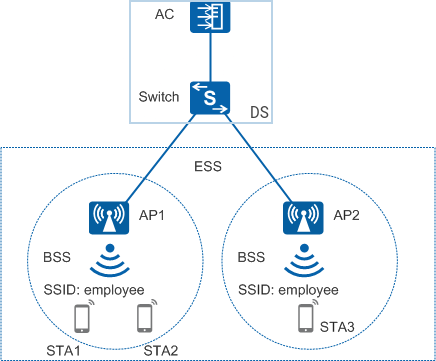
\includegraphics[width=\linewidth]{figures/terminology}
  \end{minipage}
  \hfill
  \begin{minipage}{0.5\textwidth}
    \centering
    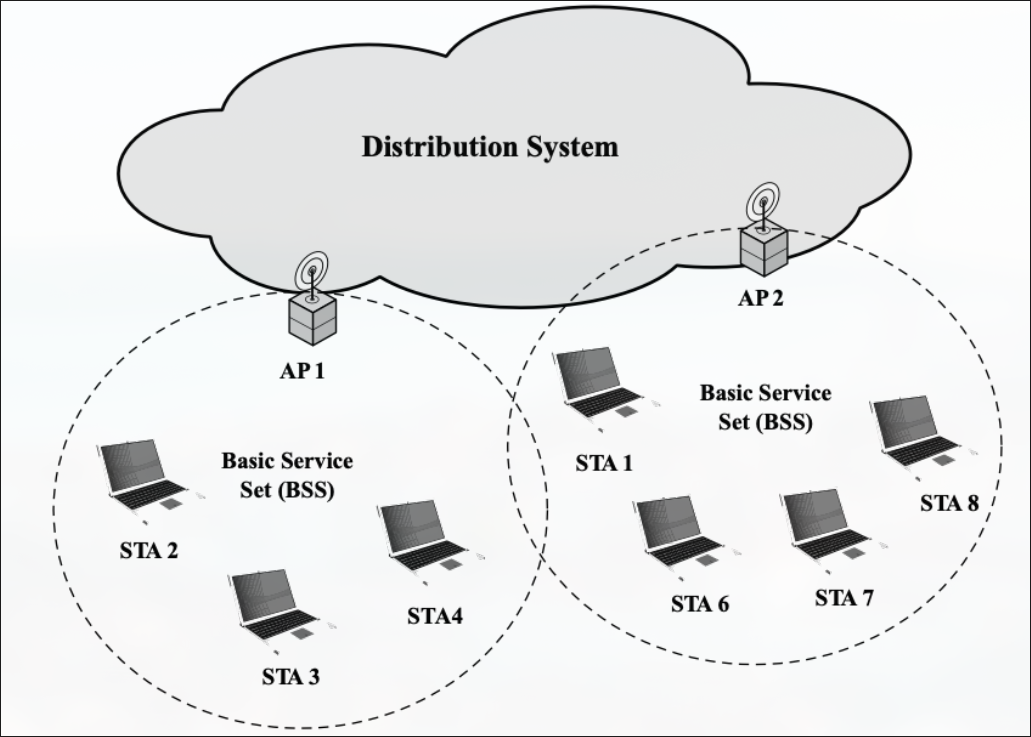
\includegraphics[width=1.1\linewidth]{figures/terminology2}
  \end{minipage}

  \begin{center}
    Networking Schema
  \end{center}
\end{figure}

\vspace{-10pt}
\begin{figure}[h]
  \begin{center}
    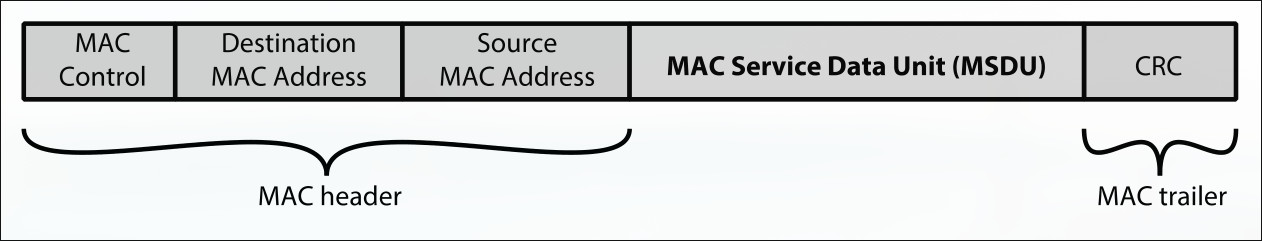
\includegraphics[width=0.6\linewidth]{figures/MPDU_format}
    \caption*{MPDU format}
  \end{center}
\end{figure}

Data are encrypted from a station to an AP, but not necessarily in the DS.

\section{802.1x Standard}

With \textbf{Wi-Fi} we mean all the certified 802.11b products, while with \textbf{Wi-Fi5} the 802.11a.

\vspace{15pt}
\begin{minipage}{0.65\textwidth}
  The IEEE 802.11 protocol stack is divided into (from top to bottom):
  \begin{itemize}
    \item \textbf{Logical Link Control}: for error and flow control.
    \item \textbf{Medium Access Control}: assembling, delivery, management and error detection of transmitted data.
    \item \textbf{Physical}: encoding/decoding of signals and bits transmission/reception.
  \end{itemize}
\end{minipage}
\hfill
\begin{minipage}{0.33\textwidth}
  \centering
  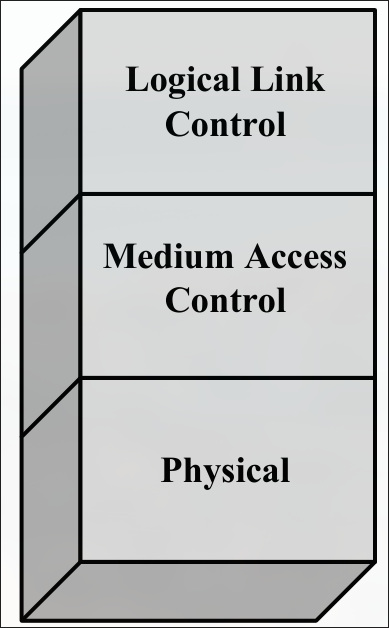
\includegraphics[width=0.5\linewidth]{figures/IEEE_stack}
\end{minipage}

\vspace{15pt}
802.11i defines the security for wireless LANs and there are 3 different instances:
\begin{itemize}
  \item \textbf{WEP} = Wired Equivalent Privacy
  \item \textbf{WPA} = Wi-Fi Protected Access
  \item \textbf{RSN} = Robust Security Network
\end{itemize}

\subsection{WEP}

Developed on the privacy portion of the 802.11, but over the years has been found several vulnerabilities.
The intention is to offer both \textbf{confidentiality} and \textbf{restriced access} of the same level of a wired connection.

It's a \textbf{symmetric key encryption} schema between host and AP where only authenticated packets can access the network, however the shared key is usually the same for all connected hosts and is not even changed frequently (often never changed). Data are encrypted at the datalink layer.

\begin{figure}[h]
  \begin{minipage}{0.46\textwidth}
    \centering
    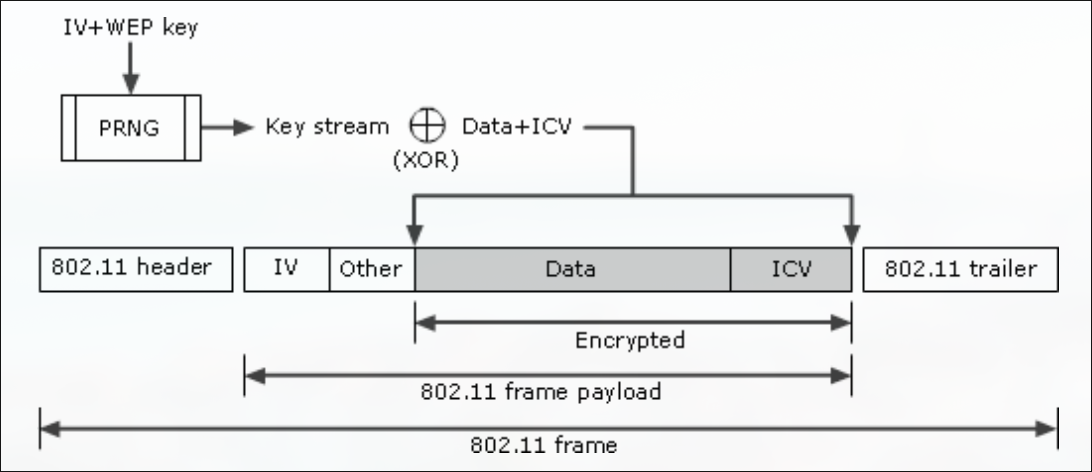
\includegraphics[width=\linewidth]{figures/WEP_encryption}
    \caption*{Encryption}
  \end{minipage}
  \hfill
  \begin{minipage}{0.52\textwidth}
    \centering
    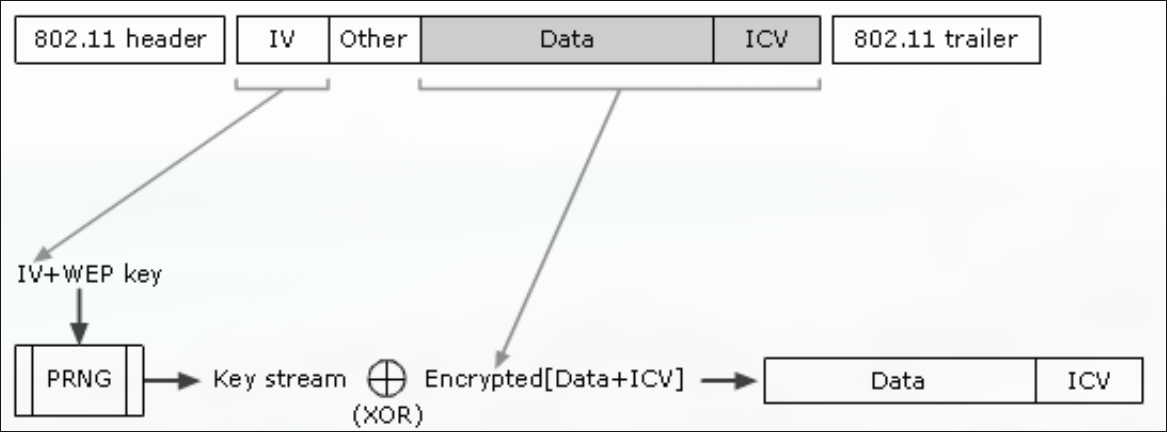
\includegraphics[width=\linewidth]{figures/WEP_decryption}
    \caption*{Decryption}
  \end{minipage}
\end{figure}

The IV is sent along the encrypted data, and as an IV it should be changed often and randomly.
However, in many WEP cards, the \textbf{IV} always starts from 0 or a pseudo-random number and then is \textbf{auto-incremented}.
This leads WEP to be vulnerable against the \textbf{Birthday attack}, where the attacker wants to find two packets encrypted with the same $(key, IV)$ pair, in order to XOR them together and with some analysis have two plaintexts.
This situation is worsened by the \textbf{key not changed} for long periods of time and with a \textbf{higher reuse of lower IVs} due to wireless card restarts.

\newpage

In fact, even with an IV pseudo-randomly initialized, the probability of finding a clash is 50\% with 4833 packets and 95\% with 10.000 ($\approx$ 15 MB), over a total pool of $2^{24} \approx 1.6 \cdot 10^6$ possible IVs.
With enough packets, an attacker is also able to \textbf{recover} the \textbf{key stream} and transmit whatever he wants.

Another vulnerability is that RC4 is weak for some IVs, and an attacker is able to recover some bytes of the key stream, and can proceed until he recovered it all.

\subsection{WPA}

Based on the current 802.11i standard, it provides mechanisms to solve most of the issues stated in 802.11, and can be seen as the patched version of WEP.

Among the patches has been added:
\begin{itemize}
  \item 4-way handshake: for mutual authentication based on a shared secret.
  \item \textbf{CCMP} (Counter-mode CBC Mac Protocol): which replaces RC4 with \textbf{AES in CTR mode}, more robust but requires new hardware. Is optional in WPA, but mandatory in WPA2.
  \item \textbf{TKIP} (Temporal Key Integrity Protocol): developed to solve the IV reuse by \textbf{generating a new password} after 10.000 packets. Is mandatory in WPA, but optional in WPA2 because later has been found vulnerable.
\end{itemize}

WPA and WPA2 admit two profiles:
\begin{itemize}
  \item \textbf{WPA-Enterprise}, which is designed to be used with 802.1x for authentication.
  \item \textbf{WPA-Personal}, that uses a PSK\footnote{Pre-Shared Key} that is usually the same for all nodes, like in WEP.
\end{itemize}

In both cases, after the authentication phase, the 4-way handshake is used to generate a session key (PTK) between each supplicant and the AP.

IV is \textbf{48 bits} long, while the key is 128 bits in WPA and \textbf{256} in WPA2.

\subsection{RSN}

Complex but final form of the 802.11i standard.

\begin{figure}[h]
  \begin{minipage}{0.48\textwidth}
    \centering
    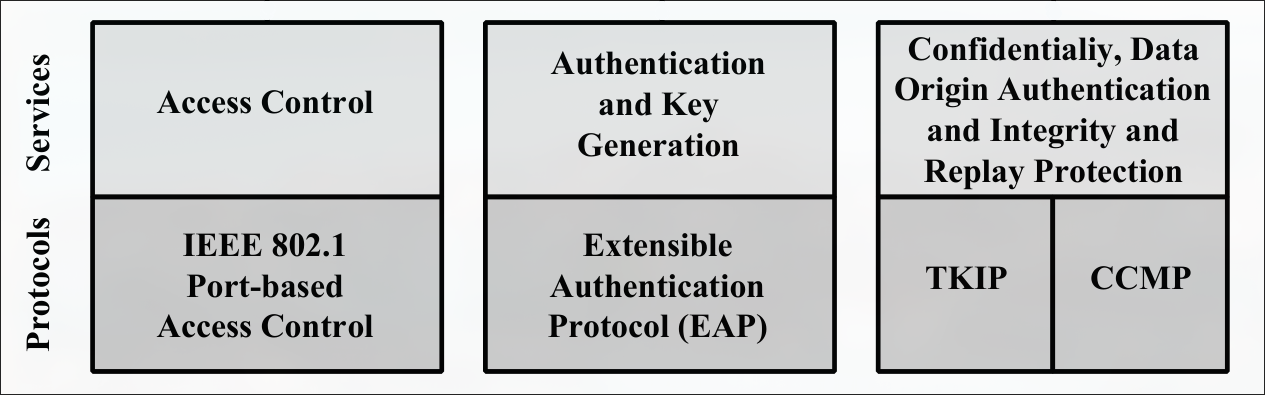
\includegraphics[width=1.1\linewidth]{figures/RSN_protocols}
    \caption*{RSN's protocols structure}
  \end{minipage}
  \quad \quad
  \begin{minipage}{0.48\textwidth}
    \centering
    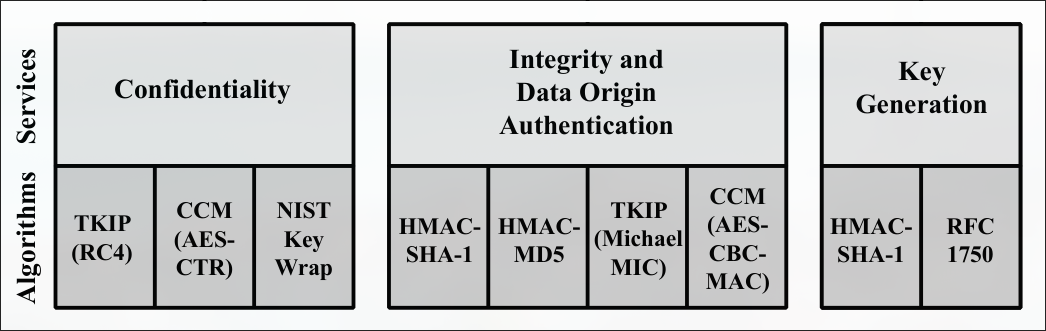
\includegraphics[width=1.085\linewidth]{figures/RSN_algorithms}
    \caption*{RSN's algorithms structure}
  \end{minipage}
\end{figure}

\newpage

RSN operation can be divided in 5 phases:
\begin{enumerate}
  \item \textbf{Discovery}: when the station \textbf{finds and chooses} an \textbf{access point}. If the access point is publicly visible, it continuously sends a \textbf{beacon} to alert the nearby devices that he's an access point and what is its SSID. Otherwise, if its hidden, the station must broadcast a \textbf{probe request} to notify its will to connect to the access point specified by its request.
  \item \textbf{Authentication}: the station connects with the authentication server, in order to \textbf{verify} its \textbf{identity}.
  \item \textbf{Key Management}: after being authenticated, the station and the authentication server exchange several messages to \textbf{set up} the \textbf{cryptographic keys}, that will be stored both in the station and the AP. This is done via the \textbf{4-way handshake}, where is confirmed the existence of the PMK, is verified the cipher spec choice and is derived a fresh PTK for the following data session.
  \item \textbf{Protected Data Transfer}: here happens the real communication from a station to another. The secure data transfer happens only between the station and the AP, who have the shared keys, so it's not an end-to-end encryption communication.
  \item \textbf{Connection Termination}: the station request the connection closure to the access point. Here the secure connection is torn down.
\end{enumerate}
The station can also be called \textbf{supplicant}.
\\\\
The most important keys are:
\begin{itemize}
  \item The \textbf{Temporal Key} is the one used with TKIP to provide confidentiality and integrity to the traffic data. The is also a variant for multicast/broadcast traffic, which is called \textbf{Group Temporal Key}.
  \item \textbf{PSK} is the Pre-Shared Key, needed to derive the \textbf{PMK}, \textit{i.e.} the Pairwise Master Key.
  \item \textbf{PTK} is the Pairwise Transient Key, is derived from the PMK and is used for the session.
\end{itemize}

In 2017 has been found an attack against the 4-way handshake, which takes the name of \textbf{KRACK} (Key Reinstallation Attack), by Vanhoef and Piessens.
This attack exploit the message retransmission, which is an allowed solution for packets loss, for reinstalling a new session key between station and access point.
Then, the attacker can
\begin{itemize}
  \item in CCMP: replay and decrypt packets.
  \item in TKIP and GCMP: replay, decrypt and even forge packets.
\end{itemize}
This vulnerability has been already patched by most vendors, but not all have yet fixed it.

\chapter{Email Security}

Despite being old the protocol is very effective.

\section{SMTP}

SMTP\footnote{Simple Mail Transfer Protocol} is text-based client-server protocol based on TCP, which has implemented its own traffic routing directly at application level.
SMTP is responsible for encapsulating the message, relaying it via multiple MTAs until reaching the destination and finally dis-encapsulating it.

The message route starts from a client, which is called \textbf{MUA} (Mail User Agent), and is used by people to connect to SMTP/ESMTP for sending/receiving messages, or for reading them via IMAP/POP.
An example of MUA are thunderbird or outlook.
Then, the client connects to a server called \textbf{MSA} (Mail Submission Agent), which in turn connects to the \textbf{MTA} (Mail Transfer Agent).
When the message reaches the receiver server \textbf{MDA} (Mail Delivery Agent), the message is saved in the \textbf{MS} (Message Store), which is continuously checked by the receiver MUA for new messages.

\begin{figure}[h]
  \begin{center}
    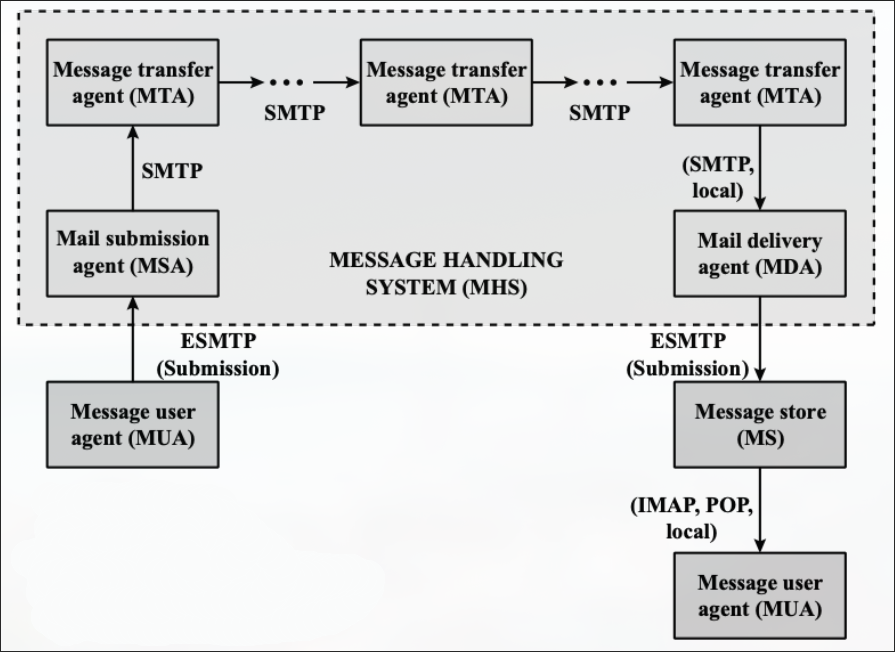
\includegraphics[width=0.7\linewidth]{figures/SMTP_schema}
    \caption*{SMTP structure}
  \end{center}
\end{figure}

\vspace{-10pt}
The MSA and MDA can read the mail content and check for spam, malware and/or control that the mail respects the required policies (\textit{e.g.} for example an organization can imply to not send attachments).

\section{IMAP/POP}

IMAP\footnote{Internet Mail Access Protocol} and POP\footnote{Post Office Protocol} are two protocols that allow a client to access/download (depending on which one of the two) the messages stored in the MS.
Both use TCP, but IMAP is more complex than POP because provides a stronger authentication in order to access the mails, while POP only download them and then delete them from the email server.

\section{Format}

\subsection{RFC 5322}

RFC 5322 defines the format for the text messages that are sent using electronic mails.
Messages are in fact encapsulated, such that the envelope contains all the information needed for transmission and delivery in its header.
The envelope remains in the layer 7 (Application) because, as we have already said, it's a complete protocol developed over the application layer.

However, due to its structure and age, SMTP has several limitations, for example
\begin{itemize}
  \item server may reject messages over a certain size
  \item cannot transmit certain national language characters
  \item cannot transmit executable files or others binaries
\end{itemize}

\subsection{MIME}

Here comes in help \textbf{MIME}\footnote{Multipurpose Internet Mail Exchange}, which is an extension of RFC 5322, intended to overcome some limitations of SMTP by encoding generic content into the standard text format.
It seems layer 6 but instead is 7.
MIME defines 5 additional layers:
\begin{enumerate}
  \item \textit{MIME-Version}
  \item \textit{Content-Type}: specifies the original data type contained in the body, \textit{e.g.} plaintext, jpeg, mpeg, $\ldots$
  \item \textit{Content-Transfer-Encoding}: specifies the encoding type used to transform the content in text compatible with mail format.
  \item \textit{Content-ID}: identify MIME entities uniquely in multiple contexts.
  \item \textit{Content-Description}: a text description useful when the object is not readable.
\end{enumerate}

\newpage

\section{Threats}

There are several threats against email security, particularly against
\begin{itemize}
  \item \textbf{Authenticity}, \textit{e.g.} unauthorized access to an enterprise's email system.
  \item \textbf{Integrity}, \textit{i.e.} unauthorized modification of email content.
  \item \textbf{Confidentiality}, \textit{i.e.} unauthorized disclosure of sensitive information.
  \item \textbf{Availability}, \textit{i.e.} prevent end users from being able to send or receive mail.
\end{itemize}

\section{Security}

\textbf{SP800-177} recommends use of a variety of standardized protocols as a means for countering threats:
\begin{itemize}
  \item \textbf{STARTTLS}: an extension of SMTP that provides authentication, integrity, non-repudiation and confidentiality for the entire MHS (Message Handling System).
  \item \textbf{S/MIME}: security enhanced MIME that provides end-to-end encryption to the body of the email, providing authentication, integrity, non-repudiation and confidentiality.
  \item \textbf{DNSSEC}\footnote{DNS Security Extensions}: extension for protecting authentication and integrity of DNS data.
  \item \textbf{DANE}\footnote{DNS-based Authentication of Named Entities}: fixes some vulnerabilities in the authentication with the certificate authority.
\end{itemize}

\begin{figure}[H]
  \begin{center}
    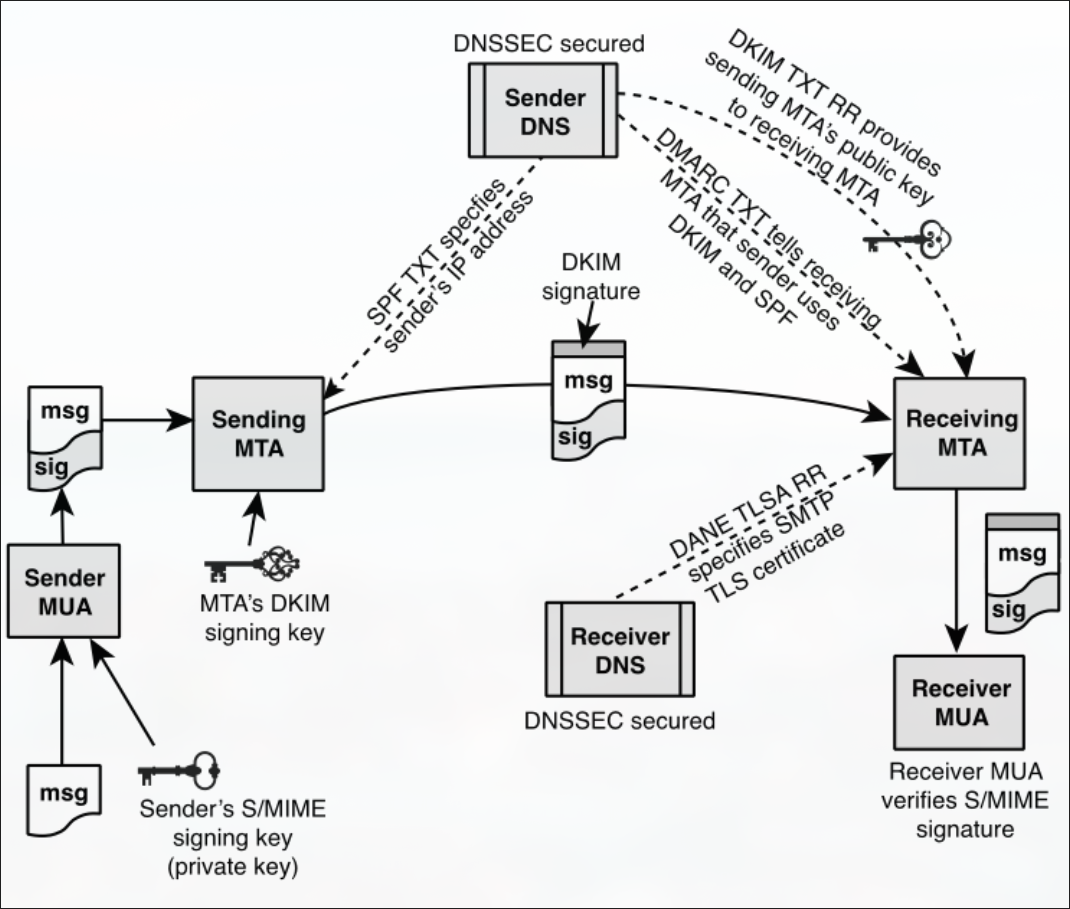
\includegraphics[width=0.7\linewidth]{figures/email_security}
  \end{center}
\end{figure}

\section{S/MIME}

\paragraph{Authentication} is provided by means of \textbf{digital signatures}: each message is hashed using \textbf{SHA-256} and the digest first encrypted using sender private key and secondly is appended to the message data.
Digital signatures provide also non-repudiation.

\paragraph{Confidentiality} is provided by message encryption, usually with \textbf{AES-128} with \textbf{CBC mode} and each key (called \textit{content-encryption key}) is only used once.
The \textbf{key itself} is also \textbf{encrypted}, usually with RSA, using the receiver's public key, and this combination of symmetric and asymmetric ciphers, allows reduced encryption/decryption times.

\begin{note}
  S/MIME, it's only a secured version of MIME, thus it manages only the email body. The header is not encrypted and can be read and also altered.
\end{note}

\vspace{5pt}
The public keys certificates used by S/MIME conform to X.509 version 3, thus S/MIME managers have to constantly update the list of trusted/untrusted certificates.
Obviously, each certificate is signed by a CA.
\\\\
RFC 2634 defines four enhanced security services for S/MIME:
\begin{itemize}
  \item Signed receipt
  \item Security labels
  \item Secure mailing list
  \item Signing certificates
\end{itemize}

\section{PEC}

Is a security enhancement to S/MIME email, which adds \textbf{non-repudiation} of recipient and \textbf{certified sending timestamp} by the server.
When the message is delivered in recipient's inbox, the sender receives a signed receipt.

Furthermore, PEC has also legal values if the servers are officially recognized.

\chapter{IP Security}

\textbf{IPsec} has been issued in 1994 by the IAB\footnote{Internet Architecture Board}, which defines the security mechanism that should be added to the level 3 of the ISO/OSI stack (IP).
Later on, with also IPv6, IPsec has become mandatory, thus every computer that implements IPv6 has also IPsec.
However, IPsec is a module thus can also be used over IPv4.
The current specification for IPsec is \textbf{RFC4301} (Security Architecture for the Internet Protocol, SAIP).
\\\\
There are two alternative extensions that implement the security transformation in IPsec:
\begin{itemize}
  \item \textbf{Authentication Header} (AH): provide message authentication.
  \item \textbf{Encapsulation Security Payload} (ESP): header and trailer are encapsulated to provide encryption and even authentication.
\end{itemize}
Furthermore, there is an auxiliary protocol called \textbf{Internet Key Exchange} (IKE), that grants a secure key exchange/setup between hosts.
\\\\
Some \textit{benefits} of IPsec are:
\begin{itemize}
  \item in a firewall/router provides \textbf{strong security to all traffic} crossing the perimeter.
  \item in a firewall/router is \textbf{resistant to bypass}.
  \item works at network level (between hosts), thus below the transport layer, thus its behavior doesn't affect the operation of above applications, nor is detected.
  \item can provide security also for individual users.
  \item implements a \textbf{secure routing architecture}.
\end{itemize}

\section{Modes}

IPsec has two working modes, which are \textbf{transport} and \textbf{tunnel}.

\begin{figure}[H]
  \begin{center}
    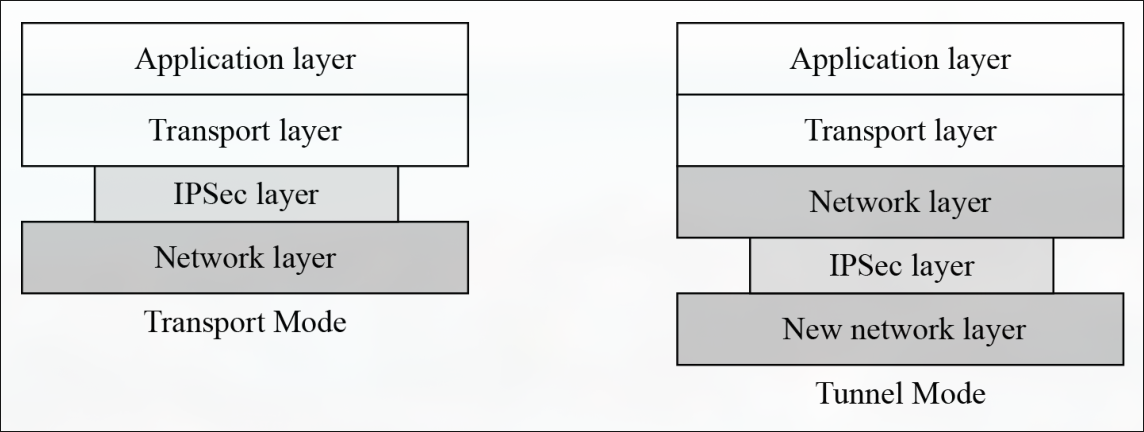
\includegraphics[width=0.7\linewidth]{figures/transport_vs_tunnel}
  \end{center}
\end{figure}

\subsection{Transport}

It provides protection for \textit{transport protocol} payloads by inserting security headers (after the original IP header and before the original IP payload).
The original IP header is not protected, but this mode is usually adopted for end-to-end communications between two hosts.

\begin{figure}[h]
  \begin{center}
    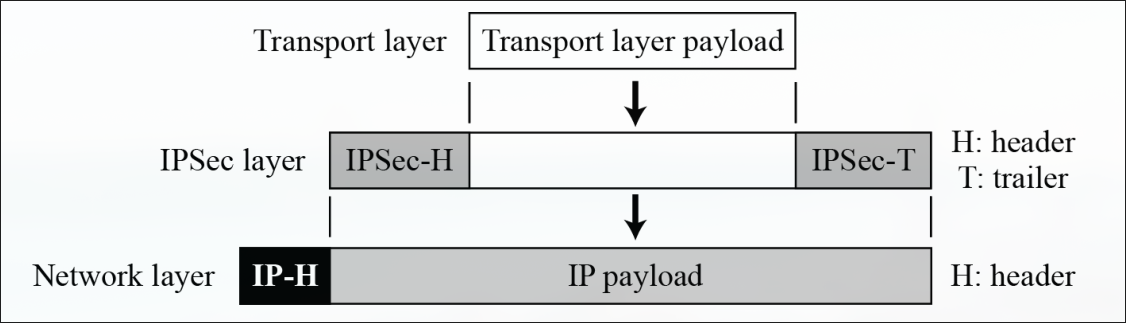
\includegraphics[width=0.8\linewidth]{figures/transport_mode}
    \caption*{Transport mode packet transformation}
  \end{center}
\end{figure}

\subsection{Tunnel}

It provides protection to the entire IP packet.
The entire packet is treated as the payload of a new packet, which will have assigned a new outer IP header.
In this way the packet structure remains standard and can be handled as a common IP packets.

This mode can be implemented if one or both ends are a security gateway, \textit{e.g.} a firewall/router that implements IPsec.
We the packet reaches the other end, it's gateway job to strip and check the IPsec data, to forward locally the original packet.

\begin{figure}[h]
  \begin{center}
    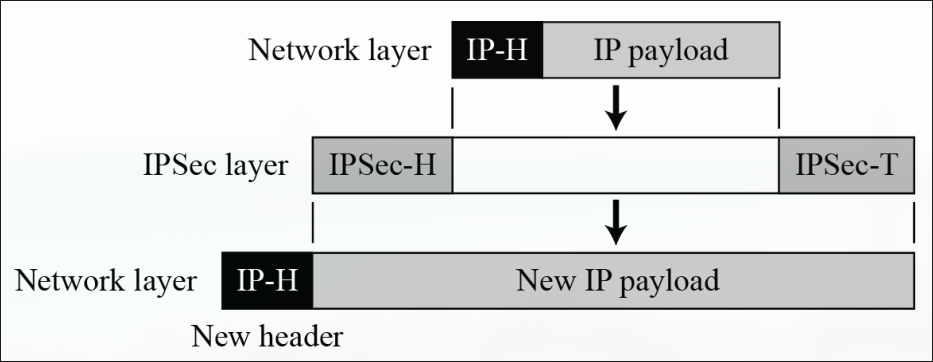
\includegraphics[width=0.65\linewidth]{figures/tunnel_mode}
    \caption*{Tunnel mode packet transformation}
  \end{center}
\end{figure}

\newpage

\section{Protocols}

ESP was designed after AH was already in use and it's like an AH enhanced version, because provides the same security functionalities plus it adds more.

In fact, they both provide
\begin{itemize}
  \item Access control
  \item Message authentication
  \item Entity authentication
  \item Replay attacks protection
\end{itemize}
but ESP also provides confidentiality.

\subsection{AH - Authenticated Header}

Is based on the use of the \textbf{MAC}, which uses SHA-1 or MD5 as hash function plus the \textbf{hosts shared key} (we recall that MAC is a keyed hash function).
Everything is left \textbf{in clear}, because AH \textbf{only adds a header} computed over the packet data (IP header, content and padding) in a way that provides both authentication and integrity of the transmitted data.

\begin{figure}[h]
  \begin{center}
    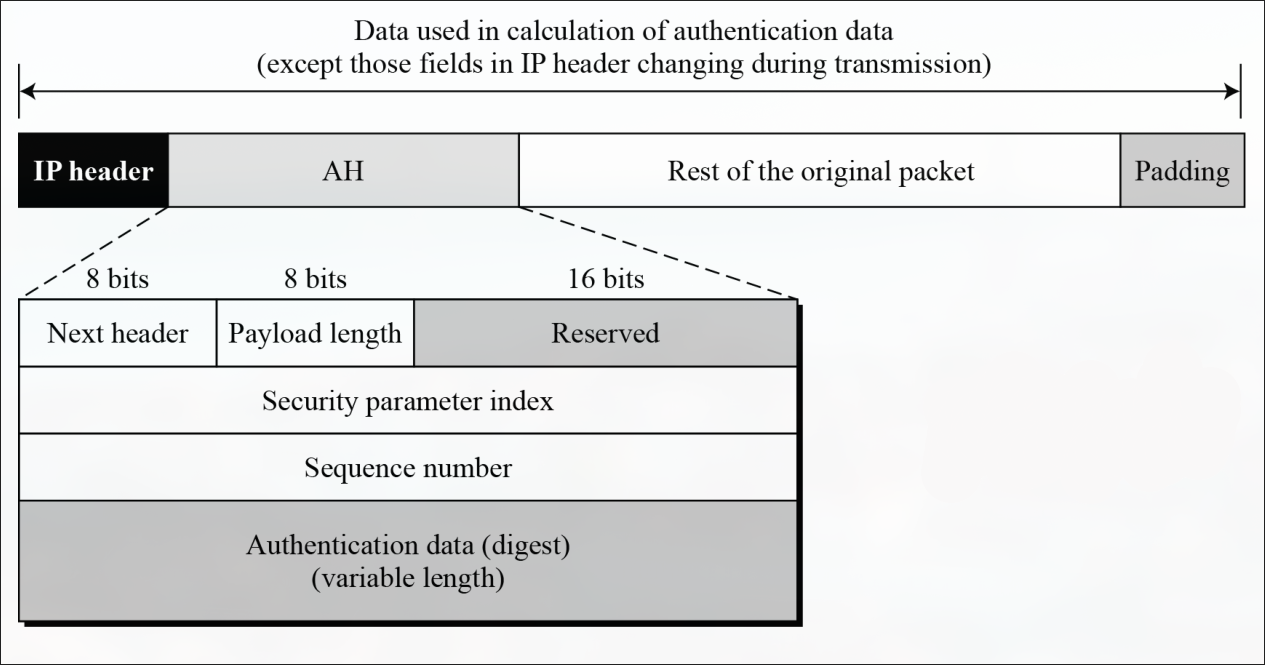
\includegraphics[width=0.95\linewidth]{figures/AH_overview}
    \caption*{New packet, after AH header is added}
  \end{center}
\end{figure}

\subsection{ESP - Encapsulating Security Payload}

Is intended to provide message content confidentiality and limited traffic flow confidentiality, but can be used also to provide authentication like AH does.
It supports a wide range of ciphers, modes and padding.

\newpage

ESP encrypts the following packet fields:
\begin{itemize}
  \item Payload Data
  \item Padding
  \item Pad Length
  \item Next Header
\end{itemize}

\begin{figure}[h]
  \begin{center}
    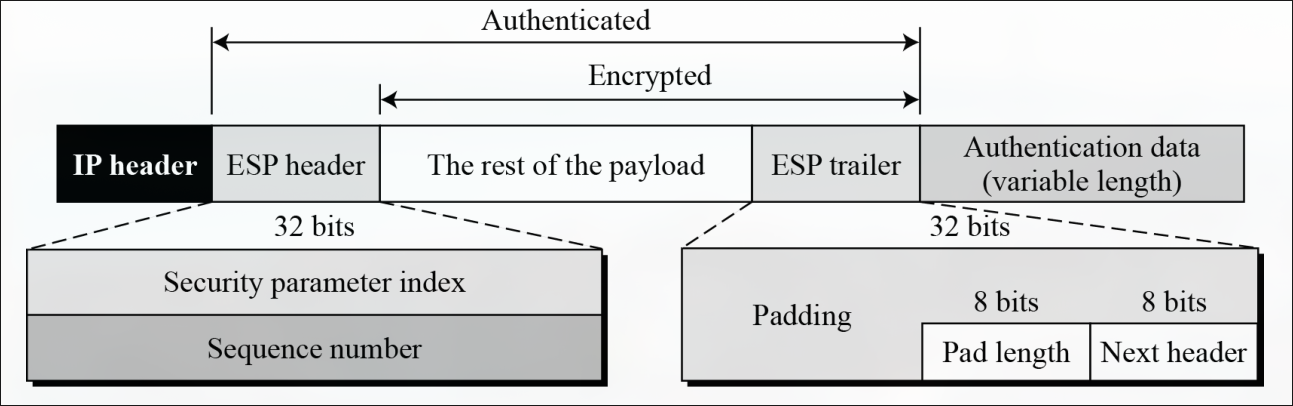
\includegraphics[width=0.9\linewidth]{figures/ESP_payload}
    \caption*{ESP payload}
  \end{center}
\end{figure}

\vspace{-10pt}
The padding field ensures that if we use a block cipher, the length is always the same no matter the plaintext length, and this assures the alignment between the fields \textit{pad length} and \textit{next header}.
It also can be used as a countermeasure to traffic analysis by adding useless padding to conceal payload's length.
\\\\
In IPsec the \textbf{sequence number} is used to decide if to accept the packet or not, as a \textbf{replay protection} and is sent in clear with the packet.
Only packets with a sequence number greater than the value stored by the host, but still within a specific window size, are accepted.
By default, the \textbf{sliding window} size is \textbf{64} and the sequence number value is in the range $[0, 2^{32} -1]$.
The sliding windows always end with the latest authenticated packet.

\begin{figure}[h]
  \begin{center}
    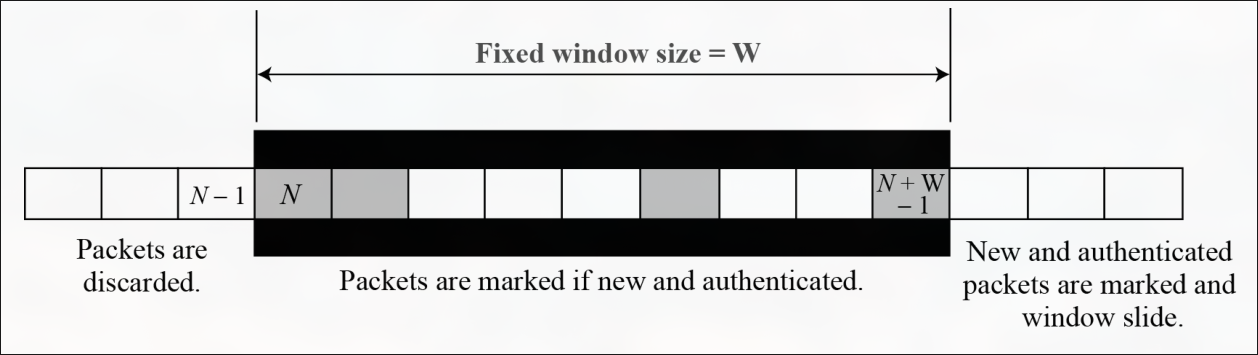
\includegraphics[width=0.9\linewidth]{figures/sequence_number}
  \end{center}
\end{figure}

The sequence number of TCP is different from IPsec sequence number.
If a packet is discarded for a certain reason and is resent, the packet remains the same with the same TCP sequence number, but the IPsec sequence number is instead updated to the latest one.

\section{SA - Security Association}

It's a \textbf{one-way} logical \textbf{relationship} between sender and receiver that affords security for the traffic carried on.
In fact, it defines the \textbf{domain of interpretation}, \textit{i.e.} all the parameters/algorithms which are used for the communication, such as:
\begin{itemize}
  \item \textbf{Security Parameters Index} (SPI)
  \item \textbf{IP Destination address}
  \item \textbf{Security Protocol Identifier}
  \item sequence number
  \item sliding window size
  \item mode (\textit{i.e.} tunnel or transport)
  \item lifetime
\end{itemize}
and many more.
\\\\
The SAD\footnote{Security Association Database} keeps track of all parameters for each index, which is a triple containing SPI, IP and protocol.
\begin{figure}[h]
  \begin{center}
    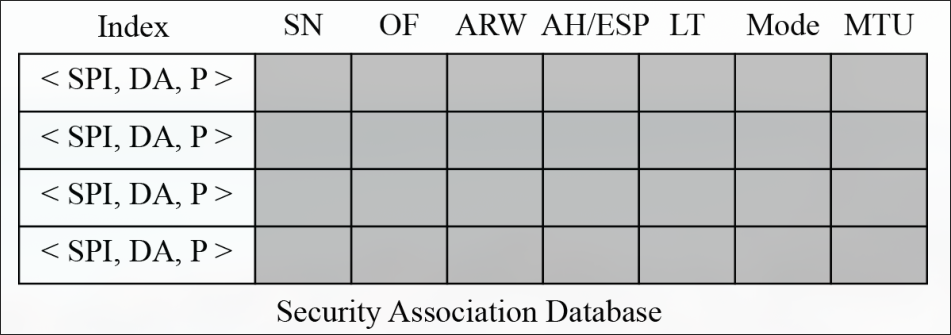
\includegraphics[width=0.7\linewidth]{figures/SAD}
  \end{center}
\end{figure}

\section{SP - Security Policy}

It's another important aspect of IPsec which defines the type of security applied to a packet when it is to be sent or when it's received, and can be compared to a packet filter (\textit{e.g.} firewall).
The SP comes first than the SA, and, depending on the policy values pre-defined by the host, each packet can either be:
\begin{itemize}
  \item \textbf{bypassed}: it means that the packet is accepted plus skips the SA control.
  \item \textbf{applied}: the packet is accepted and is relayed to the SA for a further check.
  \item \textbf{dropped}: the SP doesn't allow the packet and discards it.
\end{itemize}
The SP rules are kept in its own database (SPD), like for SA.

\end{document}
